% Created 2025-01-27 Mon 01:04
% Intended LaTeX compiler: pdflatex
\documentclass[11pt]{article}
\usepackage[utf8]{inputenc}
\usepackage[T1]{fontenc}
\usepackage{graphicx}
\usepackage{longtable}
\usepackage{wrapfig}
\usepackage{rotating}
\usepackage[normalem]{ulem}
\usepackage{amsmath}
\usepackage{amssymb}
\usepackage{capt-of}
\usepackage{hyperref}
\author{Javier Pacheco}
\date{2024-07-04}
\title{jpachecoxyz.github.io}
\hypersetup{
 pdfauthor={Javier Pacheco},
 pdftitle={jpachecoxyz.github.io},
 pdfkeywords={},
 pdfsubject={My website wrapped in an org file.},
 pdfcreator={Emacs 29.4 (Org mode 9.7.20)}, 
 pdflang={English}}
\begin{document}

\maketitle
\tableofcontents


\section{Configuration files}
\label{sec:orgf8deb39}
\subsection{Useful elisp functions \& scripts.}
\label{sec:org79c861a}
\subsubsection{publish.sh}
\label{sec:org6cb4823}
This is the script that I use to publish my web within emacs.
\begin{minted}[linenos=true,numbersep=2pt,breaklines=true,bgcolor=GreenYellow!20]{shell}

# Created By: Javier Pacheco - javier@jpacheco.xyz
# Created On: 05/07/24
# Project: Publish my blog.

# cd ~/webdev/blog/ && hugo && cd ../jpachecoxyz.github.io/ && echo "Site published correctly..." && echo "Enter your commit: "
#
# read commit && git add . && git commit -m "$commit" && echo "hit enter to continue..." && read && git push

cd ~/webdev/jpachecoxyz/ && hugo
echo "Site published correctly..."

# Use the first argument as the commit message
git add .
git commit -m "$1"
git push
\end{minted}
\subsubsection{Auto save and hugo export.}
\label{sec:orgcbec4ad}
\begin{minted}[linenos=true,numbersep=2pt,breaklines=true,bgcolor=GreenYellow!20]{elisp}
;;The first line declares where is the org file is stored, in my cases is in hugo root directory in the org folder.
(("org/"
  . ((org-mode . ((eval . (org-hugo-auto-export-mode)))))))
\end{minted}
\section{Notes}
\label{sec:orgdce5be7}
\subsection{custom hugo front-mater:}
\label{sec:org7a2c85a}
\begin{verbatim}
:EXPORT_HUGO_CUSTOM_FRONT_MATTER+: :opengraph true
\end{verbatim}
The above code generate in the markdown file the following:
\begin{minted}[linenos=true,numbersep=2pt,breaklines=true,bgcolor=GreenYellow!20]{markdown}
+++
title = "Search tool in your HUGO website."
author = ["Javier Pacheco"]
description = "Description"
date = 2024-08-25T13:10:00-05:00
tags = ["blog", "tecnology"]
draft = false
opengraph = true
+++
\end{minted}
\section{Ideas}
\label{sec:orgef0c51f}
\section{About me\hfill{}\textsc{about}}
\label{sec:orga7496fc}
Greetings! I'm Javier Pacheco, a dedicated Industrial Maintenance Engineer with a rich academic foundation from the prestigious \textbf{UTM} in \textbf{H. Matamoros Tamaulipas,Mexico}. Over the span of 12 fruitful years, I've been an integral part of the automotive industry, contributing my expertise in a multitude of critical domains.

My journey began with a profound fascination for the intricate mechanisms that power manufacturing and industrial processes. At UTM, I honed my skills, diving deep into the realms of engineering, automation, and problem-solving. This foundation paved the way for my foray into the dynamic world of industrial maintenance.

Within the automotive landscape, I've carved my niche in handling Programmable Logic Controllers (PLCs), robotics, and programming, orchestrating seamless operations and bolstering efficiency. My prowess extends beyond conventional boundaries—I harness the power of CAD software to craft intricate designs that harmonize innovation with practicality.

Programming is not just a skill set; it's an intrinsic part of my identity. The allure of languages such as Python, C, and Lisp captivates me, compelling me to unravel their complexities and harness their capabilities to engineer groundbreaking solutions.

My career is a testament to my unwavering commitment to innovation and continuous learning. Each challenge fuels my passion, propelling me to explore new horizons and revolutionize conventional practices. I thrive in environments that demand ingenuity and embrace the convergence of technology and creativity.

Beyond the technical facets, I am deeply invested in collaborative endeavors, fostering a culture of knowledge exchange and mentor-ship. I firmly believe that sharing insights and empowering others amplifies the impact of technological advancements.

See my whole information \href{file:///documents/cv.pdf}{here}.
\subsection{Where to Find Me}
\label{sec:orgb30bf79}
\begin{itemize}
\item \href{https://github.com/jpachecoxyz}{GitHub.}
\item \href{https://www.linkedin.com/in/jpachecom4/}{LinkedIn.}
\end{itemize}
\subsection{Projects that I'm currently develop.}
\label{sec:org3616d22}
\begin{itemize}
\item \href{https://github.com/engjpacheco/voidstrap}{Void linux installation script.}
\item \href{https://github.com/engjpacheco/noobemacs}{Noobemacs, a minimal emacs configuration with evil mode.}
\item \href{https://github.com/engjpacheco/pymetrics}{pymetrics, a python gui app to manage maintenance logs.}
\end{itemize}
\section{Wiki\hfill{}\textsc{wiki:personal}}
\label{sec:org7c6e8cd}
\subsection{Emacs}
\label{sec:orge4c8359}
\subsubsection{Doom Insert item.}
\label{sec:org75f1d71}
This script wast taken from \emph{doomemacs}, it basically insert a item such a heading, subheading, checkbox, etc. based on the item above.

\begin{minted}[linenos=true,numbersep=2pt,breaklines=true,bgcolor=GreenYellow!20]{common-lisp}
;;; javier_pacheco utilities.el --- Some useful utilities  -*- lexical-binding: t; -*-
(defun +org--insert-item (direction)
  (let ((context (org-element-lineage
                  (org-element-context)
                  '(table table-row headline inlinetask item plain-list)
                  t)))
    (pcase (org-element-type context)
      ;; Add a new list item (carrying over checkboxes if necessary)
      ((or `item `plain-list)
       (let ((orig-point (point)))
         ;; Position determines where org-insert-todo-heading and `org-insert-item'
         ;; insert the new list item.
         (if (eq direction 'above)
             (org-beginning-of-item)
           (end-of-line))
         (let* ((ctx-item? (eq 'item (org-element-type context)))
                (ctx-cb (org-element-property :contents-begin context))
                ;; Hack to handle edge case where the point is at the
                ;; beginning of the first item
                (beginning-of-list? (and (not ctx-item?)
                                         (= ctx-cb orig-point)))
                (item-context (if beginning-of-list?
                                  (org-element-context)
                                context))
                ;; Horrible hack to handle edge case where the
                ;; line of the bullet is empty
                (ictx-cb (org-element-property :contents-begin item-context))
                (empty? (and (eq direction 'below)
                             ;; in case contents-begin is nil, or contents-begin
                             ;; equals the position end of the line, the item is
                             ;; empty
                             (or (not ictx-cb)
                                 (= ictx-cb
                                    (1+ (point))))))
                (pre-insert-point (point)))
           ;; Insert dummy content, so that `org-insert-item'
           ;; inserts content below this item
           (when empty?
             (insert " "))
           (org-insert-item (org-element-property :checkbox context))
           ;; Remove dummy content
           (when empty?
             (delete-region pre-insert-point (1+ pre-insert-point))))))
      ;; Add a new table row
      ((or `table `table-row)
       (pcase direction
         ('below (save-excursion (org-table-insert-row t))
                 (org-table-next-row))
         ('above (save-excursion (org-shiftmetadown))
                 (+org/table-previous-row))))

      ;; Otherwise, add a new heading, carrying over any todo state, if
      ;; necessary.
      (_
       (let ((level (or (org-current-level) 1)))
         ;; I intentionally avoid `org-insert-heading' and the like because they
         ;; impose unpredictable whitespace rules depending on the cursor
         ;; position. It's simpler to express this command's responsibility at a
         ;; lower level than work around all the quirks in org's API.
         (pcase direction
           (`below
            (let (org-insert-heading-respect-content)
              (goto-char (line-end-position))
              (org-end-of-subtree)
              (insert "\n" (make-string level ?*) " ")))
           (`above
            (org-back-to-heading)
            (insert (make-string level ?*) " ")
            (save-excursion (insert "\n"))))
         (run-hooks 'org-insert-heading-hook)
         (when-let* ((todo-keyword (org-element-property :todo-keyword context))
                     (todo-type    (org-element-property :todo-type context)))
           (org-todo
            (cond ((eq todo-type 'done)
                   ;; Doesn't make sense to create more "DONE" headings
                   (car (+org-get-todo-keywords-for todo-keyword)))
                  (todo-keyword)
                  ('todo)))))))

    (when (org-invisible-p)
      (org-show-hidden-entry))
    (when (and (bound-and-true-p evil-local-mode)
               (not (evil-emacs-state-p)))
      (evil-insert 1))))

;;;###autoload
(defun +org/insert-item-below (count)
  "Inserts a new heading, table cell or item below the current one."
  (interactive "p")
  (dotimes (_ count) (+org--insert-item 'below)))

;;;###autoload
(defun +org/insert-item-above (count)
  "Inserts a new heading, table cell or item above the current one."
  (interactive "p")
  (dotimes (_ count) (+org--insert-item 'above)))


(defun org-make-olist (arg)
  (interactive "P")
  (let ((n (or arg 1)))
    (when (region-active-p)
      (setq n (count-lines (region-beginning)
                           (region-end)))
      (goto-char (region-beginning)))
    (dotimes (i n)
      (beginning-of-line)
      (insert (concat (number-to-string (1+ i)) ". "))
      (forward-line))))
\end{minted}
\subsubsection{Highlight yanked text}
\label{sec:orga7b74a9}

This function describes itself so\ldots{}
\begin{minted}[linenos=true,numbersep=2pt,breaklines=true,bgcolor=GreenYellow!20]{common-lisp}
(defun meain/evil-yank-advice (orig-fn beg end &rest args)
  (pulse-momentary-highlight-region beg end 'mode-line-active)
  (apply orig-fn beg end args))
(advice-add 'evil-yank :around 'meain/evil-yank-advice)
\end{minted}
\subsubsection{Replace '-' with '•'.}
\label{sec:orgce8c542}
\begin{minted}[linenos=true,numbersep=2pt,breaklines=true,bgcolor=GreenYellow!20]{common-lisp}
(defun jp/org-font-setup ()
  ;; Replace list hyphen with dot
  (font-lock-add-keywords 'org-mode
                          '(("^ *\\([-]\\) "
                             (0 (prog1 () (compose-region (match-beginning 1) (match-end 1) "•")))))))

(jp/org-font-setup)
\end{minted}
\subsubsection{Custom\textsubscript{id}.}
\label{sec:orgd7d8924}
\begin{minted}[linenos=true,numbersep=2pt,breaklines=true,bgcolor=GreenYellow!20]{elisp}
;;;; org-id
(declare-function org-id-add-location "org")
(declare-function org-with-point-at "org")
(declare-function org-entry-get "org")
(declare-function org-id-new "org")
(declare-function org-entry-put "org")

;; Copied from this article (with minor tweaks from my side):
;; https://writequit.org/articles/emacs-org-mode-generate-ids.html.
(defun jp/org--id-get (&optional pom create prefix)
  "Get the CUSTOM_ID property of the entry at point-or-marker POM.
If POM is nil, refer to the entry at point.  If the entry does
not have an CUSTOM_ID, the function returns nil.  However, when
CREATE is non nil, create a CUSTOM_ID if none is present already.
PREFIX will be passed through to `org-id-new'.  In any case, the
CUSTOM_ID of the entry is returned."
  (org-with-point-at pom
    (let ((id (org-entry-get nil "CUSTOM_ID")))
      (cond
       ((and id (stringp id) (string-match \\S- id))
        id)
       (create
        (setq id (org-id-new (concat prefix "h")))
        (org-entry-put pom "CUSTOM_ID" id)
        (org-id-add-location id (format "%s" (buffer-file-name (buffer-base-buffer))))
        id)))))

(declare-function org-map-entries "org")

;;;###autoload
(defun jp/org-id-headlines ()
  "Add missing CUSTOM_ID to all headlines in current file."
  (interactive)
  (org-map-entries
   (lambda () (jp/org--id-get (point) t))))

;;;###autoload
(defun jp/org-id-headline ()
  "Add missing CUSTOM_ID to headline at point."
  (interactive)
  (jp/org--id-get (point) t))
\end{minted}
\subsubsection{Add ID's to headers - Org roam.}
\label{sec:orgeb515fc}
\begin{minted}[linenos=true,numbersep=2pt,breaklines=true,bgcolor=GreenYellow!20]{common-lisp}
(defun jp/org-id-store-link-for-headers ()
  "Run `org-id-store-link' for each header in the current buffer."
  (interactive)
  (save-excursion
    (goto-char (point-min))
    (while (re-search-forward org-heading-regexp nil t)
      (org-id-store-link))))
\end{minted}
\subsubsection{Toggle org-emphasis-markers}
\label{sec:org9eb93ba}
\begin{minted}[linenos=true,numbersep=2pt,breaklines=true,bgcolor=GreenYellow!20]{elisp}
(defun jp/org-toggle-emphasis-markers (&optional arg)
  "Toggle emphasis markers and display a message."
  (interactive "p")
  (let ((markers org-hide-emphasis-markers)
        (msg ""))
    (when markers
      (setq-local org-hide-emphasis-markers nil)
      (setq msg "Emphasis markers are now visible."))
    (unless markers
      (setq-local org-hide-emphasis-markers t)
      (setq msg "Emphasis markers are now hidden."))
    (message "%s" msg)
    (when arg
      (font-lock-fontify-buffer))))
\end{minted}
\subsubsection{Insert Org's files to Outlook.}
\label{sec:org28372ee}
\begin{enumerate}
\item Export file to clipboard.
\label{sec:orgc94f635}
\begin{minted}[linenos=true,numbersep=2pt,breaklines=true,bgcolor=GreenYellow!20]{elisp}
(defun export-org-email ()
  "Export the current email org buffer and copy it to the
clipboard"
  (interactive)
  (let ((org-export-show-temporary-export-buffer nil)
        (org-html-head (org-email-html-head)))
    (org-html-export-as-html)
    (with-current-buffer "*Org HTML Export*"
      (kill-new (buffer-string)))
    (message "HTML copied to clipboard")))
(global-set-key (kbd "C-c C-x C-e") 'export-org-email)
\end{minted}
\item Add some CSS to the file.
\label{sec:org537cf71}
\begin{minted}[linenos=true,numbersep=2pt,breaklines=true,bgcolor=GreenYellow!20]{elisp}
(defun org-email-html-head ()
  "Create the header with CSS for use with email"
  (concat
   "<style type=\"text/css\">\n"
   "<!--/*--><![CDATA[/*><!--*/\n"
   (with-temp-buffer
     (insert-file-contents
      "~/.emacs.d/src/css/org2outlook.css")
     (buffer-string))
   "/*]]>*/-->\n"
   "</style>\n"))
\end{minted}
\end{enumerate}
\subsubsection{Org TODO auto update.}
\label{sec:orge7157c4}
\begin{minted}[linenos=true,numbersep=2pt,breaklines=true,bgcolor=GreenYellow!20]{common-lisp}
(defun org-todo-if-needed (state)
  "Change header state to STATE unless the current item is in STATE already."
  (unless (string-equal (org-get-todo-state) state)
    (org-todo state)))

(defun ct/org-summary-todo-cookie (n-done n-not-done)
  "Switch header state to DONE when all subentries are DONE, to TODO when none are DONE, and to DOING otherwise"
  (let (org-log-done org-log-states)   ; turn off logging
    (org-todo-if-needed (cond ((= n-done 0)
                               "TODO")
                              ((= n-not-done 0)
                               "DONE")
                              (t
                               "DOING")))))
(add-hook 'org-after-todo-statistics-hook #'ct/org-summary-todo-cookie)

(defun ct/org-summary-checkbox-cookie ()
  "Switch header state to DONE when all checkboxes are ticked, to TODO when none are ticked, and to DOING otherwise"
  (let (beg end)
    (unless (not (org-get-todo-state))
      (save-excursion
        (org-back-to-heading t)
        (setq beg (point))
        (end-of-line)
        (setq end (point))
        (goto-char beg)
        ;; Regex group 1: %-based cookie
        ;; Regex group 2 and 3: x/y cookie
        (if (re-search-forward "\\[\\([0-9]*%\\)\\]\\|\\[\\([0-9]*\\)/\\([0-9]*\\)\\]"
                               end t)
            (if (match-end 1)
                ;; [xx%] cookie support
                (cond ((equal (match-string 1) "100%")
                       (org-todo-if-needed "DONE"))
                      ((equal (match-string 1) "0%")
                       (org-todo-if-needed "TODO"))
                      (t
                       (org-todo-if-needed "DOING")))
              ;; [x/y] cookie support
              (if (> (match-end 2) (match-beginning 2)) ; = if not empty
                  (cond ((equal (match-string 2) (match-string 3))
                         (org-todo-if-needed "DONE"))
                        ((or (equal (string-trim (match-string 2)) "")
                             (equal (match-string 2) "0"))
                         (org-todo-if-needed "TODO"))
                        (t
                         (org-todo-if-needed "DOING")))
                (org-todo-if-needed "DOING"))))))))
(add-hook 'org-checkbox-statistics-hook #'ct/org-summary-checkbox-cookie)
\end{minted}
\subsubsection{Org-buffer-scratchpad.}
\label{sec:orgdea84d8}
\begin{minted}[linenos=true,numbersep=2pt,breaklines=true,bgcolor=GreenYellow!20]{common-lisp}
(defun new-scratch-pad ()
  "Create a new org-mode buffer for random stuff."
  (interactive)
  (progn
    (let ((buffer (generate-new-buffer "Org-scratch-buffer")))
      (switch-to-buffer buffer)
      (setq buffer-offer-save t)
      (org-mode)
      (olivetti-mode t))))
\end{minted}
\subsubsection{Toggle buffers.}
\label{sec:orgab83a1e}
\begin{minted}[linenos=true,numbersep=2pt,breaklines=true,bgcolor=GreenYellow!20]{common-lisp}
;; Toggle *scratch* buffer.
(defun toggle-scratch-buffer ()
  "Toggle the *scratch* buffer"
  (interactive)
  (if (string= (buffer-name) "*scratch*")
      (bury-buffer)
    (switch-to-buffer (get-buffer-create "*scratch*"))))

(defun toggle-org-buffer ()
  "Toggle the Org-scratch-buffer buffer"
  (interactive)
  (if (equal (buffer-name (current-buffer)) "Org-scratch-buffer")
      (if (one-window-p t)
          (switch-to-buffer (other-buffer))
        (delete-window))
    (if (get-buffer "Org-scratch-buffer")
        (if (get-buffer-window "Org-scratch-buffer")
            (progn
              (bury-buffer "Org-scratch-buffer")
              (delete-window (get-buffer-window "Org-scratch-buffer")))
          (switch-to-buffer "Org-scratch-buffer"))
      (new-scratch-pad))))

;; Toggle *eshell* buffer.
(defun toggle-eshell-buffer ()
  "Toggle the *eshell* buffer"
  (interactive)
  (if (string= (buffer-name) "*eshell*")
      (bury-buffer)
    (switch-to-buffer (get-buffer-create "*eshell*"))))
\end{minted}
\subsubsection{Doc at point.}
\label{sec:org031f1aa}
\begin{minted}[linenos=true,numbersep=2pt,breaklines=true,bgcolor=GreenYellow!20]{common-lisp}
(defun my-show-doc-or-describe-symbol ()
  "Show LSP UI doc if LSP is active, otherwise describe symbol at point."
  (interactive)
  (if (bound-and-true-p lsp-mode)
      (lsp-ui-doc-glance)
    (describe-symbol-at-point)))
\end{minted}
\subsubsection{Duplicate \& move up/down lines.}
\label{sec:org5313a89}
\begin{minted}[linenos=true,numbersep=2pt,breaklines=true,bgcolor=GreenYellow!20]{common-lisp}
(defun duplicate-line ()
  (interactive)
  (let ((line-text (thing-at-point 'line t)))
    (save-excursion
      (move-end-of-line 1)
      (newline)
      (insert line-text)))
  (forward-line 1))

(defun move-line-up ()
  (interactive)
  (when (not (= (line-number-at-pos) 1))
    (transpose-lines 1)
    (forward-line -2)))

(defun move-line-down ()
  (interactive)
  (forward-line 1)
  (when (not (= (line-number-at-pos) (point-max)))
    (transpose-lines 1))
  (forward-line -1))
\end{minted}
\subsubsection{Hide passwords in org files.}
\label{sec:org7f99234}
\begin{minted}[linenos=true,numbersep=2pt,breaklines=true,bgcolor=GreenYellow!20]{common-lisp}
;; Define a custom face for the highlight
(defface my-highlight-face
  '((t (:foreground "gray"))) ; Change "red" to your desired color
  "Face for highlighting !!word!! patterns.")

;; Function to replace matched text with asterisks
(defun replace-with-asterisks (limit)
  "Replace !!word!! with asterisks up to LIMIT."
  (while (re-search-forward "!!\\(.*?\\)!!" limit t)
    (let* ((match (match-string 1))
           (start (match-beginning 0))
           (end (match-end 0))
           (asterisks (make-string (length match) ?*)))
      (add-text-properties start end `(display ,asterisks face my-highlight-face)))))

;; Add custom keyword for font-lock in org-mode
(defun my/org-mode-custom-font-lock ()
  "Add custom font-lock keywords for org-mode."
  (font-lock-add-keywords nil
                          '((replace-with-asterisks))))

;; Hook the custom font-lock configuration into org-mode
(add-hook 'org-mode-hook 'my/org-mode-custom-font-lock)
\end{minted}
\subsubsection{Help at point.}
\label{sec:orgd11633a}
\begin{minted}[linenos=true,numbersep=2pt,breaklines=true,bgcolor=GreenYellow!20]{common-lisp}
(defun describe-symbol-at-point ()
  "Display the documentation of the symbol at point, if it exists."
  (interactive)
  (let ((symbol (symbol-at-point)))
    (if symbol
        (cond
         ((fboundp symbol) (describe-function symbol))
         ((boundp symbol) (describe-variable symbol))
         (t (message "No documentation found for symbol at point: %s" symbol)))
      (message "No symbol at point"))))
\end{minted}
\subsubsection{fz-themes}
\label{sec:orgb5ad0fd}
\begin{minted}[linenos=true,numbersep=2pt,breaklines=true,bgcolor=GreenYellow!20]{common-lisp}
(defun custom-jp-themes (&optional theme-dir)

  (defun custom-jp-themes (&optional theme-dir)
    "Return a list of custom themes from a specified directory.
Search the directory for files named FOO-theme.el, and return a list of FOO symbols,
excluding the 'default' theme and any internal themes.

If THEME-DIR is nil, it defaults to `~/.emacs.d/lisp/jp-themes/'."
    (let ((suffix "-theme\\.el\\'")
          (directory (or theme-dir "~/.emacs.d/lisp/jp-themes/"))
          themes)
      ;; Ensure the directory exists
      (when (file-directory-p directory)
        ;; Iterate over all theme files in the directory
        (dolist (file (directory-files directory nil suffix))
          (let ((theme (intern (substring file 0 (string-match-p suffix file)))))
            ;; Add to the list if it's valid, and exclude Emacs built-in "default" theme
            (and (not (eq theme 'default))  ;; Ensure "default" is excluded
               (not (memq theme themes))  ;; Avoid duplicates
               (push theme themes)))))
      (nreverse themes)))

  (defcustom fz-themes nil
    "List of themes (symbols or regexps) to be presented for selection.
nil shows all `custom-available-themes'."
    :type '(repeat (choice symbol regexp)))

  (defun fz-theme (theme)
    "Disable current themes and enable THEME from `fz-themes`.

The command supports previewing the currently selected theme."
    (interactive
     (list
      (let* ((regexp (consult--regexp-filter
                      (mapcar (lambda (x) (if (stringp x) x (format "\\`%s\\'" x)))
                              fz-themes)))
             (avail-themes (seq-filter
                            (lambda (x) (string-match-p regexp (symbol-name x)))
                            (custom-jp-themes)))  ;; Only use themes from custom-jp-themes
             (saved-theme (car custom-enabled-themes)))
        (consult--read
         (mapcar #'symbol-name avail-themes)
         :prompt "Theme: "
         :require-match t
         :category 'theme
         :history 'consult--theme-history
         :lookup (lambda (selected &rest _)
                   (setq selected (and selected (intern-soft selected)))
                   (or (and selected (car (memq selected avail-themes)))
                      saved-theme))
         :state (lambda (action theme)
                  (pcase action
                    ('return (fz-theme (or theme saved-theme)))
                    ((and 'preview (guard theme)) (fz-theme theme))))
         :default (symbol-name (or saved-theme 'default))))))
    (when (eq theme 'default) (setq theme nil))
    (unless (eq theme (car custom-enabled-themes))
      (mapc #'disable-theme custom-enabled-themes)
      (when theme
        (if (custom-theme-p theme)
            (enable-theme theme)
          (load-theme theme :no-confirm)))))
\end{minted}
\subsubsection{Custom functions.}
\label{sec:orgc377f74}
\begin{minted}[linenos=true,numbersep=2pt,breaklines=true,bgcolor=GreenYellow!20]{common-lisp}
;; Open files in the lisp folder
(require 'find-lisp)
(defun open-lisp-and-org-files ()
  "Open a Lisp or Org file from ~/.emacs.d/lisp directory, including subfolders."
  (interactive)
  (let* ((directory "~/.emacs.d/lisp")
         (el-files (find-lisp-find-files directory ".*\\.el$"))
         (org-files (find-lisp-find-files directory ".*\\.org$"))
         (all-files (append el-files org-files))
         (file (completing-read "Select file: " all-files nil t)))
    (find-file file)))

;; Follow urls in the buffer
(defun list-and-open-url-in-buffer ()
  "List all URLs in the current buffer, display them in the minibuffer, and open a selected URL in the browser."
  (interactive)
  (let (urls)
    (save-excursion
      (goto-char (point-min))
      (while (re-search-forward "\\(http\\|https\\|ftp\\|file\\|mailto\\):[^ \t\n]+" nil t)
        (push (match-string 0) urls)))
    (if urls
        (let ((url (completing-read "Select URL to open: " (reverse urls) nil t)))
          (browse-url url))
      (message "No URLs found in the buffer."))))

;; Export org files to pdf using tectonic
(defun org-export-to-latex-and-compile-with-tectonic ()
  "Export the current Org file to LaTeX, then compile with tectonic using shell-escape."
  (interactive)
  (let* ((org-file (buffer-file-name))
         (tex-file (concat (file-name-sans-extension org-file) ".tex"))
         (tectonic-command (concat "tectonic -Z shell-escape " tex-file)))
    ;; Export Org file to LaTeX
    (org-latex-export-to-latex)
    ;; Run tectonic command in a temporary buffer to avoid displaying the output
    (with-temp-buffer
      (shell-command tectonic-command (current-buffer)))
    (message "Compiled %s to PDF with Tectonic." tex-file)))

(global-set-key (kbd "C-c e l") 'org-export-to-latex-and-compile-with-tectonic)

;; Update my web-page
(defun publish-my-blog ()
  "Export all subtrees with Hugo, then run the publish blog script within Emacs and display a success message in the minibuffer."
  (interactive)
  (let ((commit-msg (read-string "Enter commit message: ")))
    ;; Export all subtrees with Hugo
    (org-hugo-export-wim-to-md :all-subtrees)
    ;; Run the publish script
    (let ((process (start-process-shell-command
                    "publish-blog"                       ; Process name
                    "*publish-blog-output*"              ; Output buffer
                    (format "~/webdev/jpachecoxyz.github.io/hugo/publish.sh \"%s\"" commit-msg))))  ; Run the script with the commit message
      ;; Set up the process sentinel to check the process status
      (set-process-sentinel
       process
       (lambda (process event)
         (when (string= event "finished\n")
           (message "jpacheco.xyz was correctly updated!")))))))

(global-set-key (kbd "C-c u b") 'publish-my-blog)

;; Search roam
(defun jp/search-roam ()
  "Run consult-ripgrep on the org roam directory"
  (interactive)
  (consult-ripgrep org-roam-directory nil))
(global-set-key (kbd "C-c n s") 'jp/search-roam)

(defun jp/yt-shorts-timer ()
  (interactive)
  (org-timer-set-timer "55s"))
(global-set-key (kbd "<f4>") 'jp/yt-shorts-timer)
\end{minted}
\subsection{Linux}
\label{sec:org5a1a1d2}
\subsection{Python}
\label{sec:org7f72f91}
\subsubsection{Avoid SSL verification when installing packages through pip.}
\label{sec:orgb1c9e50}
I have some issues with the firewall in one of my jobs, so in order to be able to install python packages through pip we need to skip the \texttt{SSL} verification with the following flags.
\begin{minted}[linenos=true,numbersep=2pt,breaklines=true,bgcolor=GreenYellow!20]{shell}
pip install --no-cache-dir --trusted-host pypi.org --trusted-host pypi.python.org --trusted-host files.pythonhosted.org <program>
\end{minted}
\subsection{Robots}
\label{sec:org4dc0caa}
\subsection{Windows}
\label{sec:orgc3adde9}
\subsubsection{Change IP address within terminal.}
\label{sec:orgcd758c1}
This cmd script prompt for an IP to b changed in the computer. Must run as root/administrator.
\begin{minted}[linenos=true,numbersep=2pt,breaklines=true,bgcolor=GreenYellow!20]{bat}
@echo off
setlocal

rem Prompt the user for new IP address
set /p newIP="Enter the new IP address: "
set "newSubnetMask=255.255.255.0"

rem Set the new IP address while keeping existing subnet mask and gateway
netsh interface ipv4 set address name="Ethernet" static %newIP% %newSubnetMask% 

rem Display the new IP configuration

if %errorlevel% equ 0 (
    echo IP address changed successfully.
) else (
    echo Failed to change IP address. Please make sure you have administrative privileges.
)

endlocal
\end{minted}
\section{Posts:}
\label{sec:org4d788ad}
\subsection{{\bfseries\sffamily DONE} Screen Record\hfill{}\textsc{linux:script}}
\label{sec:orgaa27a08}
This script record the screen with the \texttt{wf-recorder} tool, it can be the hole screen or a specific area of it.
The script is going to store the video in \texttt{/tmp/screencast.mp4}, this script only store one video, personally I think that have more than one record is a mess, more if you only wants to share a quick screencast to \emph{telegram, irc, cinny} or even to share it through \texttt{0x0.st}.
\subsubsection{Description and main variables:}
\label{sec:orgdd3ae36}
\begin{minted}[linenos=true,numbersep=2pt,breaklines=true,bgcolor=GreenYellow!20]{bash}
# Created By: Javier Pacheco - javier@jpacheco.xyz
# Created On: 29/03/24
# Project: Screen recorder in wayland
# Dependencies: wf-recorder wl-copy and a launcher like dmenu, fuzzel, etc.

SOUND_CARD=$(pactl list sources | awk '/Name/ && /.monitor/ {print $2}')
\end{minted}
\subsubsection{Recording functions:}
\label{sec:org9f0ec0e}
Those functions have enable the sound recording, so if you have some music, video, etc running it will record the sound but not the mic.
\begin{enumerate}
\item screencast:
\label{sec:org0740da5}
This option is going to record a specific area of the screen.
This area is going to be specified by \texttt{slurp}.
\begin{minted}[linenos=true,numbersep=2pt,breaklines=true,bgcolor=GreenYellow!20]{bash}
screencast() {
   wf-recorder --audio=$SOUND_CARD -f /tmp/screencast.mp4
}
\end{minted}
\item area:
\label{sec:orgd865e16}
This option is going to record a specific area of the screen.
This area is going to be specified by \texttt{slurp}.
\begin{minted}[linenos=true,numbersep=2pt,breaklines=true,bgcolor=GreenYellow!20]{bash}
area() {
   wf-recorder --audio=$SOUND_CARD -g "$(slurp)" -f /tmp/screencast.mp4
}
\end{minted}
\end{enumerate}
\subsubsection{Main functions:}
\label{sec:orgc09c8ca}
These functions are tools that ensures this script works correctly. For example if all ready have a existing file recorded, it will removed to record a new one, because this script only will create one video always, and also have a function to kill the process when it finished. 
\begin{enumerate}
\item check internet connection:
\label{sec:orgc168b62}
\begin{minted}[linenos=true,numbersep=2pt,breaklines=true,bgcolor=GreenYellow!20]{bash}
check_connection() {
    ping -c 1 google.com 1> /dev/null 2>&1
}
\end{minted}
\item share:
\label{sec:org89a673b}
This option is going to upload the video to \texttt{0x0.st} and copy the url to the clipboard using \texttt{wc-copy}.
\begin{minted}[linenos=true,numbersep=2pt,breaklines=true,bgcolor=GreenYellow!20]{bash}
share() {
   notify-send "uploading.." "video is upoading to 0x0.st"
   curl -F "file=@/tmp/screencast.mp4" https://0x0.st | wl-copy && notify-send "Video stored in 0x0.st"
}
\end{minted}
\item Kill existing process:
\label{sec:orgc0a9e76}
\begin{minted}[linenos=true,numbersep=2pt,breaklines=true,bgcolor=GreenYellow!20]{bash}
kill_proc(){
    pkill --signal SIGINT wf-recorder
    if [ $? -eq 0 ];
    then
        notify-send "Video stored" "Video was stored in /tmp/screencast.mp4"
        pkill --signal SIGINT wf-recorder
        exit 0
    fi
}
\end{minted}
\item Remove existing video:
\label{sec:orgaa7efb3}
\begin{minted}[linenos=true,numbersep=2pt,breaklines=true,bgcolor=GreenYellow!20]{bash}
remove_vid() {
    [ -f /tmp/screencast.mp4 ] && rm /tmp/screencast.mp4
}
\end{minted}
\end{enumerate}
\subsubsection{Sequence:}
\label{sec:orge75edc4}
This is were the scripts actually starts, first of all look if the script is already running, if not then ask for a recording option: 
\begin{minted}[linenos=true,numbersep=2pt,breaklines=true,bgcolor=GreenYellow!20]{bash}
kill_proc

OPT=$(printf "screencast\narea\nshare\nquit" | fuzzel --dmenu -p 'Select an option: ' )
case $OPT in
    'screencast')
        sleep 1
        remove_vid
        sleep 1
        screencast;;
    'area')
        sleep 1
        remove_vid
        sleep 1
        area;;
    'share') 
        check_connection && share || notify-send "Error" "check your internet connection" ;;
    *|quit) exit 0;;
esac
\end{minted}
\subsubsection{The whole code.}
\label{sec:orgbc797a0}
\begin{minted}[linenos=true,numbersep=2pt,breaklines=true,bgcolor=GreenYellow!20]{bash}
# Created By: Javier Pacheco - javier@jpacheco.xyz
# Created On: 29/03/24
# Project: Screen recorder in wayland
# Dependencies: wf-recorder wl-copy and a launcher like dmenu, fuzzel, etc.

SOUND_CARD=$(pactl list sources | awk '/Name/ && /.monitor/ {print $2}')

screencast() {
   wf-recorder --audio=$SOUND_CARD -f /tmp/screencast.mp4
}

area() {
   wf-recorder --audio=$SOUND_CARD -g "$(slurp)" -f /tmp/screencast.mp4
}

check_connection() {
    ping -c 1 google.com 1> /dev/null 2>&1
}

share() {
   notify-send "uploading.." "video is upoading to 0x0.st"
   curl -F "file=@/tmp/screencast.mp4" https://0x0.st | wl-copy && notify-send "Video stored in 0x0.st"
}

kill_proc(){
    pkill --signal SIGINT wf-recorder
    if [ $? -eq 0 ];
    then
        notify-send "Video stored" "Video was stored in /tmp/screencast.mp4"
        pkill --signal SIGINT wf-recorder
        exit 0
    fi
}

remove_vid() {
    [ -f /tmp/screencast.mp4 ] && rm /tmp/screencast.mp4
}

kill_proc

OPT=$(printf "screencast\narea\nshare\nquit" | fuzzel --dmenu -p 'Select an option: ' )
case $OPT in
    'screencast')
        sleep 1
        remove_vid
        sleep 1
        screencast;;
    'area')
        sleep 1
        remove_vid
        sleep 1
        area;;
    'share') 
        check_connection && share || notify-send "Error" "check your internet connection" ;;
    *|quit) exit 0;;
esac
\end{minted}
\subsection{{\bfseries\sffamily DONE} Efetch.el\hfill{}\textsc{emacs:script}}
\label{sec:org45010c7}
\begin{PREVIEW}
Embrace a new level of Emacs mastery with \texttt{efetch.el} – a powerful and user-friendly Emacs Fetching Tool. Designed for enthusiasts who crave insights into their Emacs environment, \texttt{efetch.el} provides a seamless way to peek under the hood of your setup. With just a simple command, unlock a left-side buffer showcasing key details such as Emacs version, host information, user details, installed packages, active theme, and default font. Customizable and accessible, this tool not only delivers a quick snapshot of your Emacs configuration but also opens the door for collaborative enhancements. Join the community on \href{https://github.com/jpachecoxyz/efetch.el}{Github} contribute your ideas, and elevate your Emacs experience with \texttt{efetch.el} today!
\end{PREVIEW}

\begin{center}
\begin{figure}[htbp]
\centering
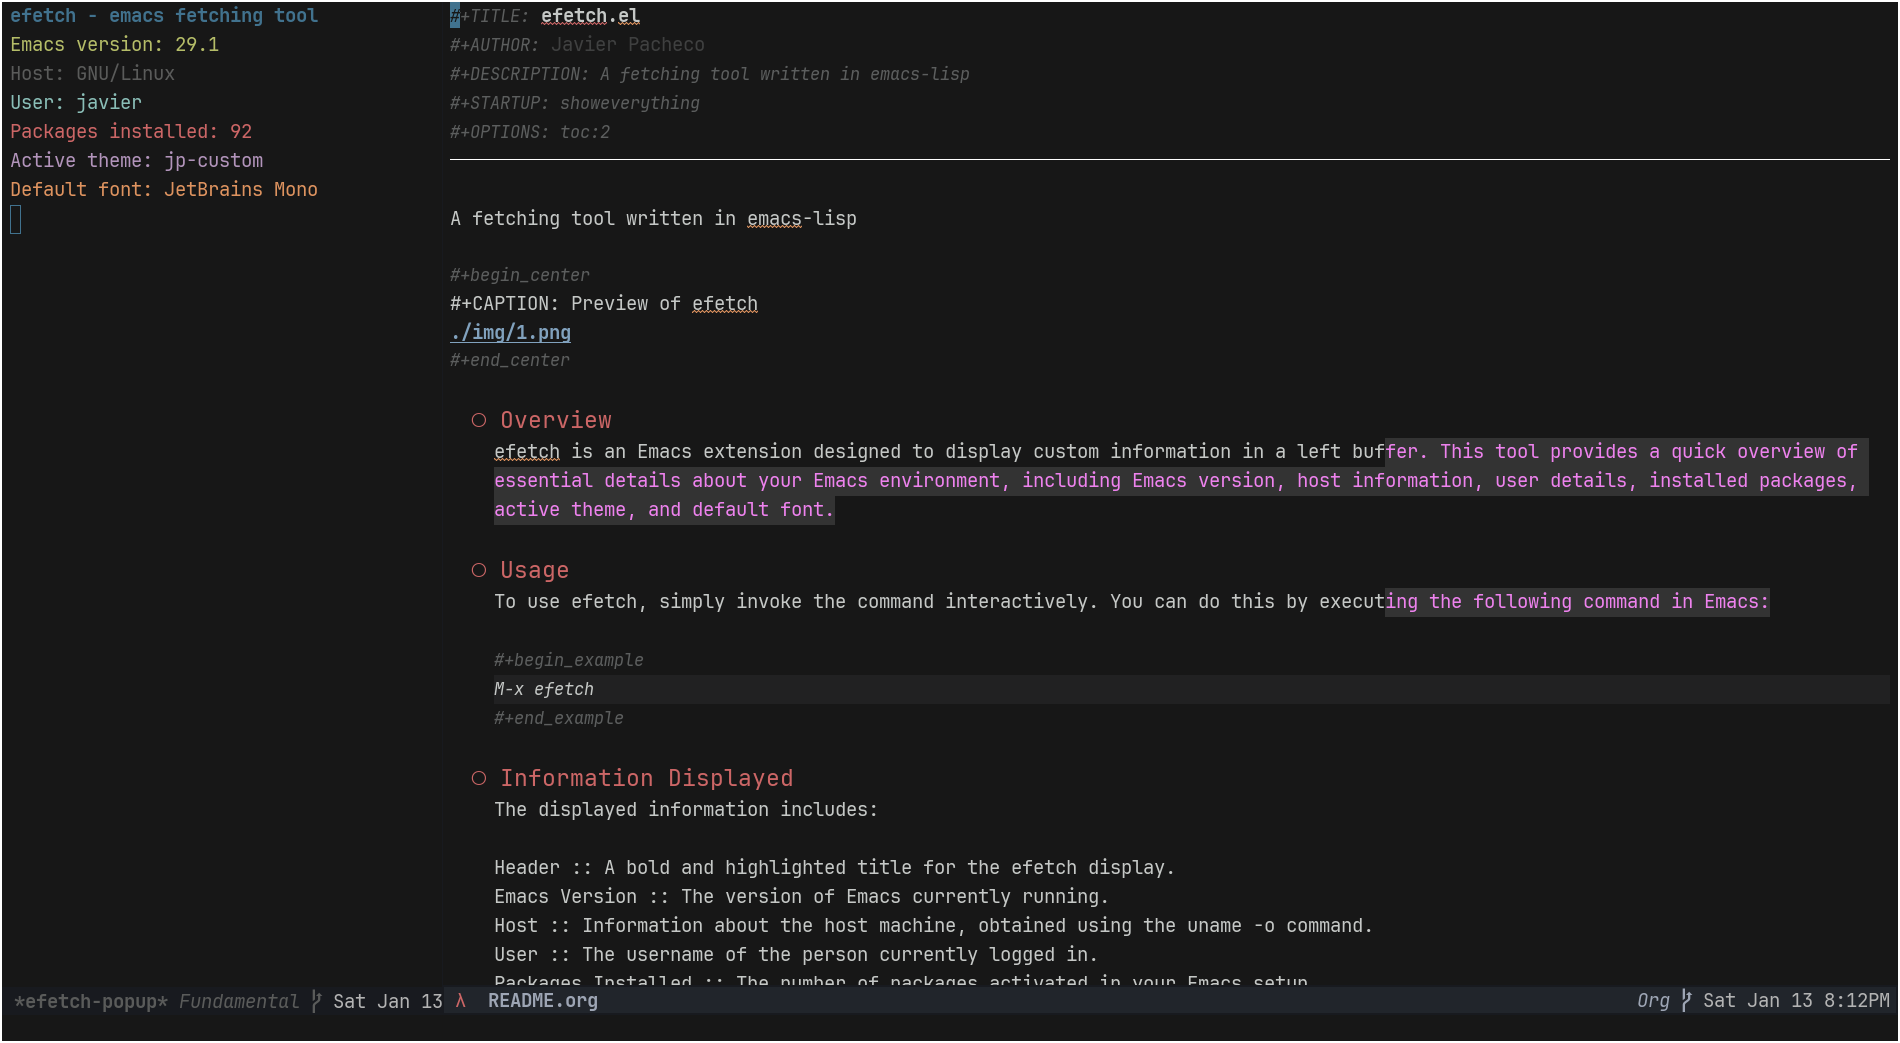
\includegraphics[width=.9\linewidth]{/images/posts/efetch.el/efetch.png}
\caption{efetch.el tool in the left side of the frame.}
\end{figure}
\end{center}
\subsubsection{Overview}
\label{sec:orga8fe2f4}
Are you an Emacs enthusiast who loves to keep track of your environment details? Look no further! We are excited to introduce \texttt{efetch.el} - the Emacs Fetching Tool. This nifty extension provides a quick and informative snapshot of your Emacs setup, helping you stay in the know about your environment configuration.
\subsubsection{Features}
\label{sec:org3f14bf9}
\begin{itemize}
\item \textbf{\textbf{Quick Access}}: Invoke \texttt{efetch} with a simple command to access a left-side buffer displaying essential information about your Emacs environment.

\item \textbf{\textbf{Information at a Glance}}: Get a concise overview, including Emacs version, host details, user information, installed packages, active theme, and default font.

\item \textbf{\textbf{Customization}}: Tailor the appearance and information displayed in the \texttt{efetch} buffer to suit your preferences.

\item \textbf{\textbf{Convenient Keyboard Shortcut}}: Close the \texttt{efetch} buffer and its window effortlessly with the \texttt{q} key.
\end{itemize}
\subsubsection{How to Use}
\label{sec:org0d09656}
\begin{enumerate}
\item \textbf{\textbf{Installation}}: Add the following line to your Emacs configuration:

\begin{minted}[linenos=true,numbersep=2pt,breaklines=true,bgcolor=GreenYellow!20]{common-lisp}
(require 'efetch)
\end{minted}
\end{enumerate}

Ensure the \texttt{efetch.el} file is in a directory included in your \texttt{load-path}.

\begin{enumerate}
\item \textbf{\textbf{Usage}}: Invoke \texttt{efetch} interactively using:
\end{enumerate}

\begin{verbatim}
M-x efetch
\end{verbatim}

The information will be displayed in a left-side buffer named \textbf{efetch-popup}.
\subsubsection{Customization}
\label{sec:orga6f059f}
Feel free to customize the appearance or the information displayed in the \texttt{efetch} buffer by modifying the relevant sections in the \texttt{efetch} function.
\subsubsection{Contribution}
\label{sec:org44585b8}
We welcome contributions and feedback! \texttt{efetch.el} is hosted on \href{https://github.com/engjpacheco/efetch.el}{github}. Feel free to \href{https://github.com/engjpacheco/efetch.el/fork}{fork the repository} and submit pull requests. 
The project is open to changes, improvements, and collaborations.
\subsubsection{Get Started}
\label{sec:orgd2df2c4}

Enhance your Emacs experience with \texttt{efetch.el}! Stay informed about your environment effortlessly. Download and integrate it into your Emacs setup today.
\subsection{{\bfseries\sffamily DONE} Void linux bootstrap.\hfill{}\textsc{linux:tecnology:script}}
\label{sec:orga890237}
\begin{PREVIEW}
This is the first post of the 2024, this is a project that I am working on in the last
year, is a minimalist voidlinux instalator it is based in some recommendations in 
a guides that some friends of my have but "semi-automated".
\end{PREVIEW}
\subsubsection{VoidStrap installer.}
\label{sec:orgea883b6}
A basic minimalist installer of \texttt{void-linux} with some packages to get ready to enjoy
this amazing GNU/Linux distribution.
\subsubsection{Usage:}
\label{sec:org99478ba}

\begin{enumerate}
\item Running install.sh
\label{sec:orgb7c1db3}

Download the iso, and once in root inside the live, git clone this repo:
(You need to update inside the iso and install \texttt{git})

NOTE: there are 3 \texttt{branches:}
\begin{description}
\item[{main}] This will install \texttt{void-musl}.
\item[{glibc}] This will install \texttt{void-glibc}.
\item[{dual}] This will install \texttt{void-glibc} dual boot with \texttt{Windows}.
\begin{itemize}
\item \textbf{This branch is tested only with \texttt{Windows}, I never try it with other distributions.}
\item If you want musl you can change the link to the mirror in the \texttt{install.sh} script:
\end{itemize}
\end{description}
\begin{verbatim}
- Change this in line 11:
export XBPS_ARCH=x86_64 && xbps-install -Suy -R http://mirrors.servercentral.com/voidlinux/current -r /mnt \
- For this:
export XBPS_ARCH=x86_64-musl && xbps-install -Suy -R http://mirrors.servercentral.com/voidlinux/current/musl -r /mnt \
\end{verbatim}

\begin{minted}[linenos=true,numbersep=2pt,breaklines=true,bgcolor=GreenYellow!20]{shell}
git clone https://git.disroot.org/jpacheco/voidstrap
cd voidstrap
sh install.sh
\end{minted}

Once there the script will open \texttt{cfdisk}, and you need to format the HDD in this 
specific format:
\begin{verbatim}
- /dev/sdX1 -> as the boot partition.
- /dev/sdY2 -> as the swap partition.
- /dev/sdZ3 -> as the root partition.
\end{verbatim}

NOTE: Replace X,Y \& Z for your partition name.
I consider to have this structure of partition, but you can change it, but you must
change the code in \texttt{postinstall.sh} when the scripts make the \texttt{fstab} archive.

\textbf{Make sure you do a backup of your files before doing crazy things and trust anyone script}

When the \texttt{install.sh} script finish, you need to run the postinstall script located in \texttt{/root folder:}
\item Running postinstall.sh
\label{sec:org34d56e4}

This script its going to create some configuration files, like: \texttt{fstab}, \texttt{rc.conf},
change the password of \texttt{root}, and add user(s).

\begin{minted}[linenos=true,numbersep=2pt,breaklines=true,bgcolor=GreenYellow!20]{shell}
xchroot /mnt
\end{minted}

Then run the \texttt{chroot.sh} script.
\begin{minted}[linenos=true,numbersep=2pt,breaklines=true,bgcolor=GreenYellow!20]{shell}
sh /root/postinstall.sh
\end{minted}

When the \texttt{postinsall.sh} script finishes, you only need to reboot and enjoy your
\textbf{Void-Linux} distribution.

When it finish you need to run the \texttt{postinstall.sh} script, that is going to install
the \textbf{X server} and some other "necessary" packages.
\end{enumerate}
\subsubsection{The custom.sh script}
\label{sec:org0836278}

This is going to install my personal dotfiles, and a specific packages that I use:
\begin{minted}[linenos=true,numbersep=2pt,breaklines=true,bgcolor=GreenYellow!20]{shell}
sh /root/custom.sh
\end{minted}

But you can specify your dotfiles repositories and others that you require whit some parameters:

\begin{verbatim}
sh custom.sh -r https://codeberg.org/jpacheco/dotfiles # specify a repo url.
sh custom.sh -p otherprogfile.csv # especify a custom package archive to install.
sh custom.sh -b dev # especify the name of a custom branch in case of needed.
\end{verbatim}
\subsubsection{References:}
\label{sec:org558d03c}
\begin{itemize}
\item \href{https://codeberg.org/jpacheco/voidstrap}{Voidstrap.}
\item \href{https://docs.voidlinux.org/}{Voidlinux Documentation.}
\item \href{https://git.disroot.org/tuxliban/tutoriales\_void/src/branch/master/Gu\%C3\%ADas}{Tuxliban guides.}
\end{itemize}
\subsection{{\bfseries\sffamily DONE} Shell-utils\hfill{}\textsc{linux:script}}
\label{sec:orgec9dddf}
\subsubsection{Overview}
\label{sec:orgb695670}
Welcome to the Shell Utilities \href{https://github.com/jpachecoxyz/shell-utils}{repository} This project provides a collection of shell scripts tailored for different window managers and environments, including i3, Hyprland, and Sway, on X11 and Wayland.
\subsubsection{Repository Structure}
\label{sec:org7d49ad1}
The repository is organized into directories based on the environment and window manager:

\begin{minted}[linenos=true,numbersep=2pt,breaklines=true,bgcolor=GreenYellow!20]{shell}
.
├── wayland
│   ├── hyprland
│   └── sway
└── x11
    └── i3
\end{minted}

\begin{description}
\item[{wayland/hyprland}] Scripts for Hyprland on Wayland.
\item[{wayland/sway}] Scripts for Sway on Wayland.
\item[{x11/i3}] Scripts for i3 on X11.
\end{description}
\subsubsection{Installation}
\label{sec:org18e1a40}
To install the scripts, use the provided \texttt{install.sh} script. You can install scripts for a specific window manager or all at once. 

NOTE: The \texttt{install.sh} scripts use \texttt{\$HOME/.local/bin} as the target, you can edit this variable inside the script, or copy the files manually somewhere as you have your path.

\begin{minted}[linenos=true,numbersep=2pt,breaklines=true,bgcolor=GreenYellow!20]{shell}
# Install scripts for a specific window manager
./install.sh sway
./install.sh hyprland
./install.sh i3

# Install all scripts
./install.sh all
\end{minted}
\subsubsection{Usage}
\label{sec:org67bc362}
Each script includes usage instructions in the comments at the top. You can run a script directly from the terminal or integrate it into your workflow.
\subsubsection{Contributing}
\label{sec:org7d38595}
We welcome contributions! If you'd like to contribute, please follow these steps:

\begin{enumerate}
\item Fork the repository.
\item Create a new branch for your feature or fix.
\item Make your changes and commit them with descriptive messages.
\item Push your changes to your fork.
\item Submit a pull request to the main repository.
\end{enumerate}
\subsubsection{Contact}
\label{sec:org8e3b04e}
For questions or suggestions, please open an issue on GitHub or contact \href{mailto:javier@jpacheco.xyz}{Javier Pacheco}.
\subsection{{\bfseries\sffamily DONE} Share Screen in Hyprland.\hfill{}\textsc{linux:wayland}}
\label{sec:orgc783128}
\subsubsection{The issue:}
\label{sec:org9c17956}
We have a telegram group, in where we share emacs things and some other related to programming and linux in the most part of the time. So one day one of the members says that we can share screens and have a kind of podcast and talk about our environment configurations (sway/hyprland), so I was very curious about it so he invite me to another telegram group, this telegram group is for his YouTube channel, for test my hyprland configuration because he told me that he has troubles in his hyprland configuration using manjaro.

Now that I face the error, I realize that in my \texttt{home-manager} compilation I had this error since I was using this tool in \texttt{nixOS}, but because I never use it, I never let it importance, so now I realize that this thing need to be solved because I going to use it in the future.

So I installed \texttt{telegram-dektop}, and try to share my configuration and guess what; yes I was unable to share my screen. It failed and pop ups some errors.
\subsubsection{Things that I try before to solve the problem.}
\label{sec:orge2eb8b4}
My main distribution at the time (2024-07-28) is \texttt{nixOS}, so I think that this could be a missing declaration in some programs, like \texttt{xdg-desktop-portal-hyprland}, because of that I was researching issues in \texttt{nixOS} \& \texttt{hyprland}, but nothing solve the problem.

So nothing that I found fix the problem, most of the issues in github was too old, or nothing to do with \texttt{nixOS}, so the last thing that I could do was compile \texttt{xdg-desktop-portal-hyprland} by source, but in \texttt{nixOS} I would install some compilers and other things that I not currently use, but it was the last option.
\subsubsection{Solving the problem.}
\label{sec:org2ae08cb}
So once in my job, with the mind more clean, I go to the hyprland \href{https://wiki.hyprland.org/Useful-Utilities/xdg-desktop-portal-hyprland/}{wiki}, and at the bottom there were some tips to debugging if some errors appears.

So I add this in my \texttt{Hyprland} configuration file:

\begin{minted}[linenos=true,numbersep=2pt,breaklines=true,bgcolor=GreenYellow!20]{conf}
exec-once = dbus-update-activation-environment --systemd --all
\end{minted}

That's it, that little command above solve my 1 day pain trying to share my screen. So I hope this little post be helpful for you if you encounter the same issue as me.

Thanks for read me.
\subsection{{\bfseries\sffamily DONE} Pymetrics\hfill{}\textsc{linux:tecnology:wayland}}
\label{sec:org724736a}
\subsubsection{Overview}
\label{sec:org484e0d8}
Managing and monitoring the performance of industrial machines is critical to ensuring minimal downtime and maximizing productivity. The need for an effective system to store and analyze maintenance data became apparent when the maintenance manager contacted me with a specific problem. They struggled to create KPI graphs because they lacked a proper system to store all the necessary data. To address this challenge, I developed a maintenance log app that efficiently tracks and records machine failures, repair time, shutdown time, and the technicians involved in the repairs. The data is stored in a CSV format, making it easy to create KPI (Key Performance Indicator) graphs in Excel for analysis.
\subsubsection{Features}
\label{sec:orga4f514a}
\begin{description}
\item[{Machine Failure Logging}] Record each instance of machine failure with timestamps.
\item[{Repair Time Tracking}] Log the start and end times of repairs to calculate the total repair duration.
\item[{Shutdown Time Monitoring}] Track the total time a machine is down due to failures and repairs.
\item[{Technician Assignment}] Assign technicians to specific repair tasks and log their involvement.
\end{description}
\subsubsection{How the Project Started}
\label{sec:org13859be}
The project began when the maintenance manager reached out to me with a significant issue: they were unable to create KPI graphs due to the lack of a system for storing maintenance data. Understanding the importance of this data for monitoring machine performance, I developed the maintenance log app in Python to solve the problem. By providing a structured way to capture and store all relevant data, the app enables easy analysis and KPI generation.
\subsubsection{Benefits}
\label{sec:orgff7c856}
The maintenance log app provides several key benefits:
\begin{itemize}
\item \textbf{Enhanced Data Management:} All data is stored in a standardized CSV format, which can be easily imported into Excel for further analysis.
\item \textbf{Improved KPI Tracking}: By analyzing the recorded data, maintenance teams can generate KPI graphs in Excel to monitor performance metrics such as Mean Time to Repair (MTTR) and Mean Time Between Failures (MTBF).
\item \textbf{Informed Decision-Making:} The insights gained from the KPI graphs help in making informed decisions to improve machine reliability and reduce downtime.
\end{itemize}
\subsubsection{Technical Details}
\label{sec:org23a0210}
The app is built using Python, leveraging its robust data handling capabilities. The CSV format is chosen for its simplicity and compatibility with various data analysis tools.
\subsubsection{Usage}
\label{sec:orgeb811bd}
The application is designed to be user-friendly, requiring minimal input from the maintenance team. The data entry process is streamlined, allowing technicians to quickly log failures and repairs without interrupting their workflow.

\begin{center}
\begin{figure}[htbp]
\centering
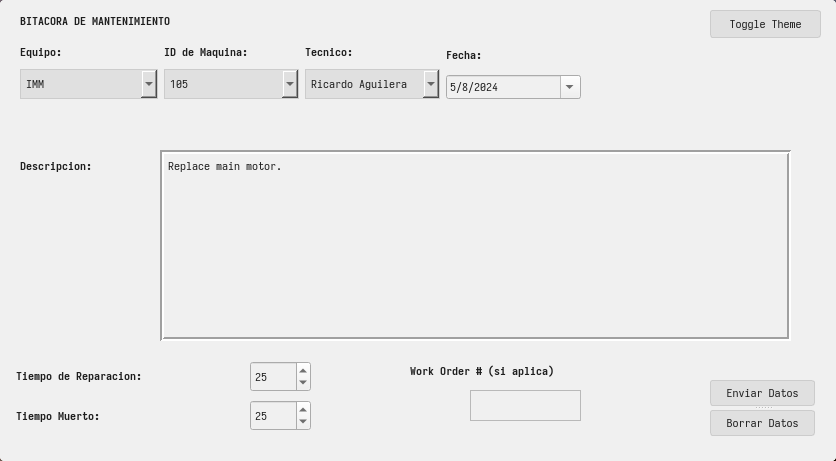
\includegraphics[width=.9\linewidth]{/images/posts/pymetrics/pymetrics.png}
\caption{Pymetrics in light-mode.}
\end{figure}
\end{center}
\subsubsection{How to Get Started}
\label{sec:org3fa8642}
You can access the source code and instructions for setting up the maintenance log app on GitHub: \href{https://github.com/jpachecoxyz/pymetrics}{Pymetrics Repository}.
\subsubsection{Conclusion}
\label{sec:org602162b}
This maintenance log app is a practical tool for any industrial maintenance team looking to improve their machine monitoring and maintenance processes. By providing a clear view of machine performance through KPI graphs, it helps teams identify trends and make data-driven decisions. The app was born out of a real-world need, and I'm excited to see how it can help others in similar situations.

Feel free to explore the project and contribute to its development by visiting the \href{https://github.com/jpachecoxyz/pymetrics}{Pymetrics Repository} on GitHub.
\subsection{{\bfseries\sffamily DONE} Emacs vs Neovim\hfill{}\textsc{emacs:tecnology}}
\label{sec:orgc4cc718}
\subsubsection{Neovim for Programming}
\label{sec:org58c0514}
\begin{itemize}
\item Efficiency and Speed: Neovim is highly efficient for programming due to its lightweight nature and focus on speed. It starts up faster and can handle large files with ease.
\item Plugin Ecosystem: Neovim has a rich plugin ecosystem, especially for programming-related tasks. Plugins like nvim-treesitter for syntax highlighting, telescope.nvim for fuzzy finding, and coc.nvim or nvim-lspconfig for Language Server Protocol (LSP) support make it a powerful choice for coding.
\item Modal Editing: Neovim, like Vim, uses modal editing, which can be very powerful for code navigation and manipulation once you get used to it.
\end{itemize}
\subsubsection{Emacs for Writing Posts (and Beyond)}
\label{sec:orgfeabf94}
\begin{itemize}
\item Org-mode: Emacs shines when it comes to writing and organizing content, especially with Org-mode. Org-mode is exceptional for note-taking, task management, and writing posts or documentation. It allows you to export your work to various formats (HTML, PDF, \LaTeX{}, etc.) easily.
\item Extensibility: Emacs is known for its extensibility. You can customize it to be a full-fledged IDE, text editor, or writing tool. For blog posts, especially if you're using something like ox-hugo, Emacs can be incredibly powerful.
\item Unified Environment: If you prefer an environment where you can write, code, manage tasks, and do everything in one place, Emacs offers that. It's an all-in-one tool where you can manage your entire workflow.
\end{itemize}
\subsubsection{Which Should You Choose?}
\label{sec:org58de4d6}
\begin{itemize}
\item For Programming: Neovim might be better if you want a focused, fast, and highly efficient tool purely for coding. It's especially suitable if you prefer modal editing and a streamlined environment.

\item For Writing and More: Emacs could be better if you're looking for a versatile tool that excels at writing posts, organizing content, and managing your entire workflow beyond just coding. It's particularly strong if you take advantage of Org-mode's features.
\end{itemize}

Since I already use Emacs for my blog with Hugo, I find it more productive to keep using it for writing and content management while possibly using Neovim for coding tasks if you prefer its efficiency and speed.
\subsection{{\bfseries\sffamily DONE} How I made my blog with emacs and hugo\hfill{}\textsc{emacs:tecnology:personal}}
\label{sec:orgdf88df7}
\begin{PREVIEW}
I have been using emacs most of the time for writting, and of course when I started to make my blog I have been use it (emacs) since of it. In the beginig when I start writing I was using some scripts and tips from \href{https://systemcrafters.net/}{system crafters} he use htmlize and some \emph{lisp} scripting. It was ok but then I have been watching some \href{https://www.youtube.com/@LukeSmithxyz}{lukesmith} videos and see this \href{https://www.youtube.com/watch?v=jAXKSKb3etk\&pp=ygUOaHVnbyBsdWtlc21pdGg\%3D}{video} about him switching to \texttt{HUGO}, so I decided to check \texttt{HUGO} too.
\end{PREVIEW}

\begin{center}
\begin{figure}[htbp]
\centering
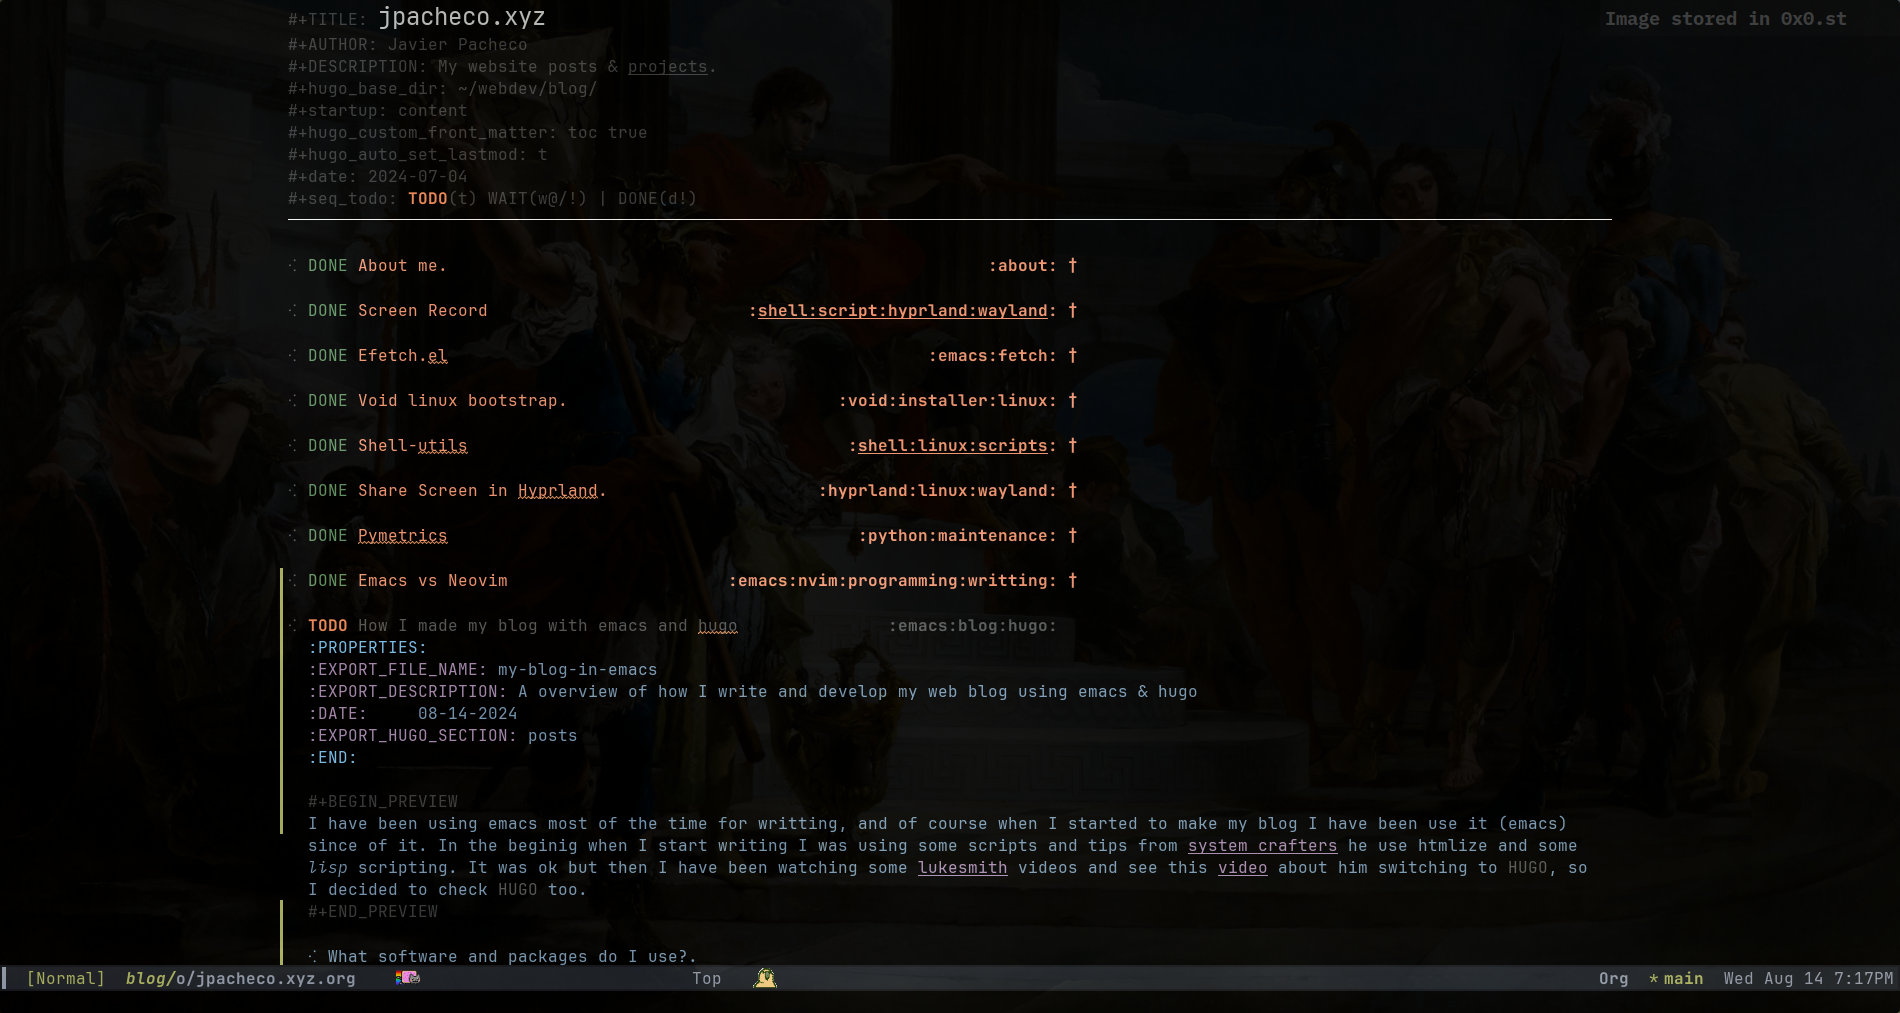
\includegraphics[width=.9\linewidth]{/images/posts/my-blog-in-emacs/overview.png}
\caption{A overview of how my org file looks like.}
\end{figure}
\end{center}
\subsubsection{What software and packages do I use?.}
\label{sec:orgd149edd}
Yep! I use \texttt{emacs} 🤓 and \texttt{ox-hugo}.

And to build the static web I use \href{https://gohugo.io/getting-started/quick-start/}{HUGO} and \texttt{git}.
\begin{listing}[htbp]
\begin{minted}[linenos=true,numbersep=2pt,breaklines=true,bgcolor=GreenYellow!20]{elisp}
(use-package ox-hugo
  :ensure t
  :after ox)
\end{minted}
\caption{This is what I have in my emacs configuration.}
\end{listing}
\subsubsection{Org and its configuration.}
\label{sec:org3eb15b2}
\texttt{HUGO} uses markdown to manage the sites, posts, etc. but because we where using emacs, (we don't like others than org syntax), so there are a lot of variables that \texttt{ox-hugo} handle in order to been exported to markdown syntax.

In my case I like to develop my whole blog into a single org-file

\begin{listing}[htbp]
\begin{minted}[linenos=true,numbersep=2pt,breaklines=true,bgcolor=GreenYellow!20]{elisp}
#+begin_src org
#+TITLE: jpacheco.xyz
#+AUTHOR: Javier Pacheco
#+DESCRIPTION: My website posts & projects.
#+hugo_base_dir: ~/webdev/blog/
#+startup: content
#+hugo_custom_front_matter: toc true
#+hugo_auto_set_lastmod: t
#+date: 2024-07-04
#+seq_todo: TODO(t) WAIT(w@/!) | DONE(d!)
\end{minted}
\caption{My metadata in my org-file.}
\end{listing}
---

These are the most important and relevant to use within HUGO:

\begin{itemize}
\item \emph{\#+HUGO\textsubscript{BASE}\textsubscript{DIR}:}
\end{itemize}
This declare where you HUGO site is located, basically in the path where you run \texttt{hugo new site my-site}.
\begin{itemize}
\item \emph{\#+HUGO\textsubscript{CUSTOM}\textsubscript{FRONT}\textsubscript{MATTER}}:
\end{itemize}
This is for enable/disable the toc of the posts when ox-hugo exported to md format.
\subsubsection{Writing the posts.}
\label{sec:orgd7bba3a}
Write a post is very easy to start, you only need to add a org lvl-1 header, and add a more metadata (properties). The sub-headers of the post are going to be org-lvl-3 headers, and so on.

\begin{listing}[htbp]
\begin{minted}[linenos=true,numbersep=2pt,breaklines=true,bgcolor=GreenYellow!20]{org}
* TODO How I made my blog with emacs and hugo               :emacs:blog:hugo:
   :PROPERTIES:
   :EXPORT_FILE_NAME: my-blog-in-emacs
   :EXPORT_DESCRIPTION: A overview of how I write and develop my web blog using emacs & hugo
   :DATE:     08-14-2024
   :EXPORT_HUGO_SECTION: posts
   :END:
\end{minted}
\caption{Example of an article.}
\end{listing}
---

\begin{itemize}
\item \emph{:EXPORT\textsubscript{FILE}\textsubscript{NAME}}:
\end{itemize}
This is how your file is going to be stored, you may or not add the \texttt{.md} extension.
\begin{itemize}
\item \emph{:EXPORT\textsubscript{HUGO}\textsubscript{SECTION}}:
\end{itemize}
Here is the tricky part, if you have multiple sections like: post, projects, topics, etc. this is where the file is going to be stored.

If the sub-header starts with a TODO, when exported the md metadata is going to have \texttt{draftt: true}, which means even the archive is going to be created when you run hugo to create your site that md archive is going to be ignored until you finish (remove the TODO or change it to DONE.).

And that's it, you can search more options for manage the front matter in hugo in this \href{https://ox-hugo.scripter.co/}{page.}

Thanks for reading.
\subsection{{\bfseries\sffamily DONE} Install Telega in NixOS - Emacs.\hfill{}\textsc{emacs:linux:tecnology}}
\label{sec:org1915b50}
What is telega?.
---
According to the \href{https://github.com/zevlg/telega.el}{Github} repository:
\begin{description}
\item[{Telega}] telega.el is full featured unofficial client for Telegram platform for GNU Emacs.
\end{description}

---

As you may know, my main OS, at this time (2024-08-21) is \texttt{NixOS}, so I was trying to install \texttt{Telega} in my emacs, but as you can imagine, the file system hierarchy don't works "normal" in \texttt{NixOS}, so is a little tricky set up the environment to actually make \texttt{Telega} works.
\subsubsection{Requisites:}
\label{sec:orge61b678}
\begin{itemize}
\item gnumake. (To compile).
\item cmake (To compile).
\item tdlib (Version > 1.8.29).
\end{itemize}
\subsubsection{Process of installation.}
\label{sec:org5b3888c}
\begin{enumerate}
\item install the dependencies using your \texttt{configuration.nix}, \texttt{home-manager}, or wathever method you use to install packages in \texttt{NixOS}.
\item Install Telega in emacs.
\begin{listing}[htbp]
\begin{minted}[linenos=true,numbersep=2pt,breaklines=true,bgcolor=GreenYellow!20]{elisp}
(use-package telega
:ensure t)
\end{minted}
\caption{Example of telega installation unsing use-package.}
\end{listing}
\item Now, because I use \texttt{NixOS} (by the way), you must know that the file system hierarchy don't works same as in linux or macOS, so I need to declare where telega is going to see the \texttt{tdlib} libraries, so:
\begin{minted}[linenos=true,numbersep=2pt,breaklines=true,bgcolor=GreenYellow!20]{elisp}
(setq telega-server-lib-prefix "/home/user/.nix-profile/")
\end{minted}
\item Compile Telega-server inside emacs.
\begin{verbatim}
M-x telega-server-build
\end{verbatim}

Or simply run telega:
\begin{verbatim}
M-x telega
\end{verbatim}
\end{enumerate}

With that, Telega must be compiled, and ready to go.
\subsection{{\bfseries\sffamily DONE} Search tool in your HUGO website.\hfill{}\textsc{blog:tecnology}}
\label{sec:orgba330bc}
As websites grow, incorporating a search feature becomes increasingly crucial. However, implementing search functionality can be challenging on a statically generated site since there's no server-side component to handle the search. Instead, the search must be performed on the client side within the browser using JavaScript.

\begin{center}
\begin{figure}[htbp]
\centering

\includegraphics[width=.9\linewidth]{/images/posts/hugo-search/jpacheco-search.png}
\caption{This is how my web looks.}
\end{figure}
\end{center}

Fortunately, there are existing solutions to address this issue. Below, we demonstrate one such solution that utilizes FuseJS and MarkJS. This implementation is inspired by a gist from eddiewebb, but it's built using plain JavaScript rather than jQuery.
\subsubsection{Page - content/search/\textsubscript{index.md}}
\label{sec:org0e2fdc5}
Create a page to serve as the search form and display search results. In the markdown, set the layout to ‘search’ and proceed to create this layout (in the next step) to easily manage the HTML.

\begin{minted}[linenos=true,numbersep=2pt,breaklines=true,bgcolor=GreenYellow!20]{markdown}
---
title: "Search"
sitemap:
  priority : 0.1
layout: "search"
---
\end{minted}
\subsubsection{Layout - layout/\textsubscript{default}/search.html}
\label{sec:org698261e}
This search page contains a <div> element for displaying search results (\#search-results) and another <div> element for showing a loading message (.search-loading). The layout also defines a template that will later be used in the JavaScript to render a single search result. Finally, it loads the necessary JS libraries (from a CDN in this example, though self-hosting is an option).

\begin{minted}[linenos=true,numbersep=2pt,breaklines=true,bgcolor=GreenYellow!20]{html}
{{ define "main" }}

<main>
    <form action="/search" method="GET">
        <input type="search" name="q" id="search-query" placeholder="Search...." autofocus>
        <!-- <button type="submit">Search</button> -->
    </form>
    <div id="search-results"></div>
    <div class="search-loading">Loading...</div>

    <script id="search-result-template" type="text/x-js-template">
    <div id="summary-${key}">
        <h3><a href="${link}">${title}</a></h3>
        <p>${snippet}</p>
        <p>
            <small>
                ${ isset tags }Tags: ${tags}<br>${ end }
            </small>
        </p>
    </div>
    </script>

    <script src="https://cdnjs.cloudflare.com/ajax/libs/fuse.js/6.6.2/fuse.min.js" integrity="sha512-Nqw1tH3mpavka9cQCc5zWWEZNfIPdOYyQFjlV1NvflEtQ0/XI6ZQ+H/D3YgJdqSUJlMLAPRj/oXlaHCFbFCjoQ==" crossorigin="anonymous" referrerpolicy="no-referrer"></script>

    <script src="https://cdnjs.cloudflare.com/ajax/libs/mark.js/8.11.1/mark.min.js" integrity="sha512-5CYOlHXGh6QpOFA/TeTylKLWfB3ftPsde7AnmhuitiTX4K5SqCLBeKro6sPS8ilsz1Q4NRx3v8Ko2IBiszzdww==" crossorigin="anonymous" referrerpolicy="no-referrer"></script>
</main>

{{ end }}
\end{minted}
\subsubsection{JS}
\label{sec:org50f026a}
The main part of the code is JavaScript, where everything is tied together. The URL parameters are read to obtain the query, which is then passed to FuseJS and MarkJS, and the results are written back to the page.

\begin{minted}[linenos=true,numbersep=2pt,breaklines=true,bgcolor=GreenYellow!20]{javascript}
var summaryInclude = 180;
var fuseOptions = {
    shouldSort: true,
    includeMatches: true,
    includeScore: true,
    tokenize: true,
    location: 0,
    distance: 100,
    minMatchCharLength: 1,
    keys: [
        {name: "title", weight: 0.45},
        {name: "contents", weight: 0.4},
        {name: "tags", weight: 0.1},
        {name: "categories", weight: 0.05}
    ]
};

// =============================
// Search
// =============================

var inputBox = document.getElementById('search-query');
if (inputBox !== null) {
    var searchQuery = param("q");
    if (searchQuery) {
        inputBox.value = searchQuery || "";
        executeSearch(searchQuery, false);
    } else {
        document.getElementById('search-results').innerHTML = '<p class="search-results-empty">Please enter a word or phrase above, or see <a href="/tags/">all tags</a>.</p>';
    }
}

function executeSearch(searchQuery) {

    show(document.querySelector('.search-loading'));

    fetch('/index.json').then(function (response) {
        if (response.status !== 200) {
            console.log('Looks like there was a problem. Status Code: ' + response.status);
            return;
        }
        // Examine the text in the response
        response.json().then(function (pages) {
            var fuse = new Fuse(pages, fuseOptions);
            var result = fuse.search(searchQuery);
            if (result.length > 0) {
                populateResults(result);
            } else {
                document.getElementById('search-results').innerHTML = '<p class=\"search-results-empty\">No matches found</p>';
            }
            hide(document.querySelector('.search-loading'));
        })
        .catch(function (err) {
            console.log('Fetch Error :-S', err);
        });
    });
}

function populateResults(results) {

    var searchQuery = document.getElementById("search-query").value;
    var searchResults = document.getElementById("search-results");

    // pull template from hugo template definition
    var templateDefinition = document.getElementById("search-result-template").innerHTML;

    results.forEach(function (value, key) {

        var contents = value.item.contents;
        var snippet = "";
        var snippetHighlights = [];

        snippetHighlights.push(searchQuery);
        snippet = contents.substring(0, summaryInclude * 2) + '&hellip;';

        //replace values
        var tags = ""
        if (value.item.tags) {
            value.item.tags.forEach(function (element) {
                tags = tags + "<a href='/tags/" + element + "'>" + "#" + element + "</a> "
            });
        }

        var output = render(templateDefinition, {
            key: key,
            title: value.item.title,
            link: value.item.permalink,
            tags: tags,
            categories: value.item.categories,
            snippet: snippet
        });
        searchResults.innerHTML += output;

        snippetHighlights.forEach(function (snipvalue, snipkey) {
            var instance = new Mark(document.getElementById('summary-' + key));
            instance.mark(snipvalue);
        });

    });
}

function render(templateString, data) {
    var conditionalMatches, conditionalPattern, copy;
    conditionalPattern = /\$\{\s*isset ([a-zA-Z]*) \s*\}(.*)\$\{\s*end\s*}/g;
    //since loop below depends on re.lastInxdex, we use a copy to capture any manipulations whilst inside the loop
    copy = templateString;
    while ((conditionalMatches = conditionalPattern.exec(templateString)) !== null) {
        if (data[conditionalMatches[1]]) {
            //valid key, remove conditionals, leave contents.
            copy = copy.replace(conditionalMatches[0], conditionalMatches[2]);
        } else {
            //not valid, remove entire section
            copy = copy.replace(conditionalMatches[0], '');
        }
    }
    templateString = copy;
    //now any conditionals removed we can do simple substitution
    var key, find, re;
    for (key in data) {
        find = '\\$\\{\\s*' + key + '\\s*\\}';
        re = new RegExp(find, 'g');
        templateString = templateString.replace(re, data[key]);
    }
    return templateString;
}

// Helper Functions
function show(elem) {
    elem.style.display = 'block';
}
function hide(elem) {
    elem.style.display = 'none';
}
function param(name) {
    return decodeURIComponent((location.search.split(name + '=')[1] || '').split('&')[0]).replace(/\+/g, ' ');
}

// Keybinds functions
document.addEventListener('keydown', function(event) {
    // Check if the Windows key (or Command key on macOS) and forward slash are pressed
    if (event.metaKey && event.key === '/') {
        // Prevent the default action if necessary
        event.preventDefault();

        // Navigate to the search page
        window.location.href = '/search';

        // Wait for the page to load and then focus on the search input
        window.addEventListener('load', function() {
            const searchInput = document.getElementById('search-query');
            if (searchInput) {
                searchInput.focus();
            }
        });
    }
});
\end{minted}
\subsubsection{The Data - layouts/\textsubscript{default}/index.json}
\label{sec:orgb9bacfa}
All the work we’ve done up until now has been front-end workings, but we also need to build an index.json file which will act as our data source (which is fetched from the JS).

\begin{minted}[linenos=true,numbersep=2pt,breaklines=true,bgcolor=GreenYellow!20]{json}
{{- $.Scratch.Add "index" slice -}}
{{- range .Site.RegularPages -}}
    {{- $.Scratch.Add "index" (dict "title" .Title "tags" .Params.tags "categories" .Params.categories "contents" .Plain "permalink" .Permalink) -}}
{{- end -}}
{{- $.Scratch.Get "index" | jsonify -}}
\end{minted}
\subsubsection{Conclusion}
\label{sec:org5198d48}
You can extend this further by offering a live search preview, adding more filters, or allowing sorting options. This method provides a powerful and flexible way to implement search functionality on a static site without relying on any backend services.
\subsection{{\bfseries\sffamily DONE} Basics of HUGO\hfill{}\textsc{blog:personal:tecnology}}
\label{sec:org9a4bac8}
\subsubsection{Introduction}
\label{sec:org1465eee}
\begin{quote}
"Hugo is one of the most popular open-source static site generators. With its amazing speed and flexibility, Hugo makes building websites fun again."
\end{quote}
\subsubsection{Installation}
\label{sec:org0e34b12}
Hugo is multi platform, so the installation depends on what SO do you use, in this example I Show how to install in \texttt{Arch-linux} because it's easy.

\begin{minted}[linenos=true,numbersep=2pt,breaklines=true,bgcolor=GreenYellow!20]{shell}
sudo pacman -S hugo
\end{minted}
\subsubsection{Creating a New Site}
\label{sec:orge7e38e4}
\begin{enumerate}
\item Initialize a New Hugo Site
\label{sec:orgfdc11a6}
This is the command in order to create a hugo site,

\begin{minted}[linenos=true,numbersep=2pt,breaklines=true,bgcolor=GreenYellow!20]{shell}
hugo new site my-website.org
\end{minted}

\begin{description}
\item[{my-website.org}] is the name of the directory that hugo is going to create, and where all the files are going to be.
\end{description}
\item Directory Structure Overview
\label{sec:org755fc01}
\begin{verbatim}
$ tree -d my-website.org

my-website.org
├── archetypes
├── assets
├── content
├── data
├── i18n
├── layouts
├── static
└── themes
\end{verbatim}
\item Initialize an empty git repository.
\label{sec:org6747b8f}

This is very useful because in case of mess, you can easily roll back.
\begin{minted}[linenos=true,numbersep=2pt,breaklines=true,bgcolor=GreenYellow!20]{shell}
git init
\end{minted}
\end{enumerate}
\subsubsection{Creating Content}
\label{sec:org33f857f}
\begin{enumerate}
\item Creating a New Post
\label{sec:orge02d3e4}
This is the command to create post within HUGO:

\begin{minted}[linenos=true,numbersep=2pt,breaklines=true,bgcolor=GreenYellow!20]{shell}
hugo new content content/posts/my-first-post.md
\end{minted}

Hugo creates a \texttt{my-first-post.md} in the \texttt{content/posts/} directory, open it with your editor, you must see this content in the file:

\begin{minted}[linenos=true,numbersep=2pt,breaklines=true,bgcolor=GreenYellow!20]{markdown}
+++
title = 'My First Post'
date = 2024-01-14T07:07:07+01:00
draft = true
+++
\end{minted}

Notice the draft value in the front matter is true. By default, Hugo does not publish draft content when you build the site. Learn more about draft, future, and expired content.

Add some Markdown to the body of the post, but do not change the draft value.

\begin{minted}[linenos=true,numbersep=2pt,breaklines=true,bgcolor=GreenYellow!20]{markdown}
+++
title = 'My First Post'
date = 2024-01-14T07:07:07+01:00
draft = true
+++
## Introduction

This is **bold** text, and this is *emphasized* text.

Visit the [Hugo](https://gohugo.io) website!
\end{minted}
\end{enumerate}
\subsubsection{Working with Themes}
\label{sec:org1635a98}
To install a theme is basically download it from \texttt{GitHub}, you can find more themes \href{https://themes.gohugo.io/themes}{here}.
\begin{enumerate}
\item Downloading and Installing a Theme
\label{sec:orgc73df9b}

In this guide we are going to use \texttt{PaperMod} theme, so we need to install it througt various ways.
\begin{itemize}
\item As a submodule (recommended).
\end{itemize}

\begin{minted}[linenos=true,numbersep=2pt,breaklines=true,bgcolor=GreenYellow!20]{shell}
git submodule add --depth=1 https://github.com/adityatelange/hugo-PaperMod.git themes/PaperMod
git submodule update --init --recursive # needed when you reclone your repo (submodules may not get cloned automatically)
\end{minted}

\begin{itemize}
\item Simply clone.
\end{itemize}

\begin{minted}[linenos=true,numbersep=2pt,breaklines=true,bgcolor=GreenYellow!20]{shell}
git clone https://github.com/adityatelange/hugo-PaperMod themes/PaperMod --depth=1
\end{minted}

\textbf{Keep in mind that if you clone the repository you must delete the \texttt{.git} folder inside the theme, because is going to have conflicts when you try to push your site.}

The next ones I never used, but you can go to the HUGO documentation for read more about these.
\begin{itemize}
\item Expand Method 3 - Download an unzip
\item Hugo module
\end{itemize}
\item Configuring the Theme \& see it in action.
\label{sec:org5d9e60c}
Finally set theme as PaperMod in your site config, \texttt{hugo.toml} or \texttt{config.toml}

\begin{minted}[linenos=true,numbersep=2pt,breaklines=true,bgcolor=GreenYellow!20]{toml}
theme = "PaperMod"
\end{minted}

Once you do this you can verify if the site applied the theme correctly by running the hugo server:
\begin{minted}[linenos=true,numbersep=2pt,breaklines=true,bgcolor=GreenYellow!20]{shell}
hugo server
\end{minted}
Now, in your \texttt{browser}, open \texttt{localhost:1313}, and you should see your site with the proper theme applied.
\end{enumerate}
\subsubsection{Configuration example for PaperMod theme.}
\label{sec:orgf0b5a54}
This is a basic configuration template for PaperMod theme:

\begin{minted}[linenos=true,numbersep=2pt,breaklines=true,bgcolor=GreenYellow!20]{toml}
baseURL = 'https://example.org/'
languageCode = 'en-us'
title = 'My New Hugo Site'
theme = "PaperMod"

copyright = "[PaperMod Contributors](https://github.com/adityatelange/hugo-PaperMod/graphs/contributors)"
paginate = 5
enableInlineShortcodes = true
enableRobotsTXT = true
buildDrafts = false
buildFuture = false
buildExpired = false
enableEmoji = true
pygmentsUseClasses = true
mainsections = [ "posts", "papermod" ]

[minify]
disableXML = true

[languages.en]
languageName = "English"
weight = 1

  [languages.en.taxonomies]
  category = "categories"
  tag = "tags"
  series = "series"

[[languages.en.menu.main]]
name = "Archive"
url = "archives"
weight = 5

[[languages.en.menu.main]]
name = "Posts"
url = "posts/"
weight = 10

[outputs]
home = [ "HTML", "RSS", "JSON" ]

[params]
env = "production"
description = "Theme PaperMod - https://github.com/adityatelange/hugo-PaperMod"
author = "Theme PaperMod"
defaultTheme = "auto"
ShowShareButtons = true
ShowReadingTime = true
displayFullLangName = true
ShowPostNavLinks = true
ShowBreadCrumbs = true
ShowCodeCopyButtons = true
ShowRssButtonInSectionTermList = true
ShowAllPagesInArchive = true
ShowPageNums = true
ShowToc = true
images = [ "images/papermod-cover.png" ]

  [params.profileMode]
  enabled = false
  title = "PaperMod"
  imageUrl = "#"
  imageTitle = "my image"

    [[params.profileMode.buttons]]
    name = "Archives"
    url = "archives"

    [[params.profileMode.buttons]]
    name = "Tags"
    url = "tags"

  [params.homeInfoParams]
  Title = "PaperMod's Demo"
  Content = """
?? Welcome to demo page of Hugo's theme PaperMod!
- **PaperMod**  is designed to be clean and simple but fast and responsive theme with useful feature-set that enhances UX.
- Feel free to show your support by giving us a star ?? on GitHub and sharing with your friends and social media .
- PaperMod is based on theme [Paper](https://github.com/nanxiaobei/hugo-paper/tree/4330c8b12aa48bfdecbcad6ad66145f679a430b3).
"""

  [[params.socialIcons]]
  name = "github"
  title = "View Source on Github"
  url = "https://github.com/adityatelange/hugo-PaperMod"

  [[params.socialIcons]]
  name = "Discord"
  title = "Join discord community"
  url = "https://discord.gg/ahpmTvhVmp"

  [[params.socialIcons]]
  name = "X"
  title = "Share PaperMod on X/Twitter"
  url = "https://x.com/intent/tweet/?text=Checkout%20Hugo%20PaperMod%20%E2%9C%A8%0AA%20fast,%20clean,%20responsive%20Hugo%20theme.&url=https://github.com/adityatelange/hugo-PaperMod&hashtags=Hugo,PaperMod"

  [[params.socialIcons]]
  name = "KoFi"
  title = "Buy me a Ko-Fi :)"
  url = "https://ko-fi.com/adityatelange"

  [params.assets]
  disableHLJS = true

[markup.goldmark.renderer]
unsafe = true

[markup.highlight]
noClasses = false

[services.instagram]
disableInlineCSS = true

[services.twitter]
disableInlineCSS = true
\end{minted}
\subsubsection{Building the Site}
\label{sec:org2643074}
\begin{enumerate}
\item Generating the Static Site
\label{sec:org68afc26}
At this point we need to generate the static we site, the most basic command to publish it is just run \texttt{hugo} in the terminal inside the root of the project.
So you notice that a \texttt{public} folder is now created, if you look inside, you'll find all the html files, and everything to deploy as a web page.
\item Set specific folder to export your site.
\label{sec:org6b72fa2}
If you don't want to have your publish site in the \texttt{public} folder, you can set another path to export it instead of the \texttt{public} folder by adding this line at top of your \texttt{hugo.toml} configuration file:

\begin{minted}[linenos=true,numbersep=2pt,breaklines=true,bgcolor=GreenYellow!20]{toml}
publishDir = "/path/to/export/"
#example
publishDir = "~/my-site.org/"
\end{minted}
\end{enumerate}
\subsubsection{Conclusion}
\label{sec:org67b39a6}
With all the context before, you may be able to start your web site, blog, etc. As you read, is very simple to have a very nice and useful static web-page, the "hard" part is to select the theme.

The next step is to publish your web to a custom server or on github, gitlab, codeberg pages.
\begin{enumerate}
\item Preparing for Deployment.
\item Deploying to a Web Server or Hosting Service.
\end{enumerate}
\begin{enumerate}
\item Additional Resources
\label{sec:orgf3ee645}
\begin{enumerate}
\item \href{https://gohugo.io/getting-started/quick-start/}{Hugo quick start guide.}
\item \href{https://gohugo.io/documentation/}{Hugo documentation.}
\end{enumerate}
\end{enumerate}
\subsection{{\bfseries\sffamily DONE} A job history.\hfill{}\textsc{blog:personal}}
\label{sec:org2ac081b}
\subsubsection{A brief Introduction.}
\label{sec:org25ce1bc}
This is no t going to be a post about programming or technology, this is kind of a way to express my feelings about one important thing that I think is going to change my life, I'm talking about my job and how this ambient change my mind and my vision about this important thing that a lot of us need to do and hold the job pressure to keep some security for our families.
\subsubsection{The history\ldots{}}
\label{sec:org006b20b}
I have almost 5 years working in \texttt{Autoliv} in H.Matamoros, in the meaning of that time I was trying every single day to make my best, trying to improve things, make the process better, being the fastest troubleshooting solver, have less machines failures, less downtime, questioning about how maintenance can be better, and more thing related to the maintenance department.

As you may wonder, yes, I am a maintenance technician in the die-cast area, I always though that for require something you need to share something first, so that was basically what I was doing for about 4 years, mean while in those years, I prof myself, and prof others that I was capable to have an engineering position, because I was doing some specific tasks and covering the Controls Engineer when he was out of the job, develop projects, etc, all of that being a maintenance technician. So with that being said, I apply to various engineering vacancy's, but for one reason I never have been promoted, always have other person or the manager cancel the vacant. 

That's the \texttt{why} I realize that I don't need to effort my self to achieve something that is not going  to happens. So I decide to only do the job for what I was hired (maintenance technician). 

In the past 4 and a half years, I think I was doing a good job, not because I say it, my boss say it, the engineering department say it, the production department trust in my skills as a troubleshooting resolver. So at that time I was thinking that if I was doing a “good” job, maybe it could be easy to achieve some engineering charge, the thing is that I was \texttt{wrong}. It seems that being good and give some extra skills to the job were not enough. job, maybe it could be easy to achieve some engineering charge, the thing is that I was \texttt{wrong}. It seems that be good and give some extra skills to the job were not enough.

To the time, I decided to apply to a engineering position, so I do, I have a couple of interviews with the managers, but unfortunately, they choose other person, or canceled the job position. That basically drop me down, because It was kind of I don't know, It seems that I'm was good, but not enough, some times when I fill the job when the control's engineer was out of the job, I have treat with others engineers, but I don't want to say bad things about them, but in my perspective, those engineers are too young and with a lack of experience, don't let me wrong, but is I went messed up when those guys came to me and ask me for directions, while technically I am a low level in the structure:
\begin{quote}
Engineer > Technician
\end{quote}

So I remember that day, I returned to my home so mad and sad, Why?, a few weeks before, I was working in the first shift, everything goes fine, I have like 5 months since I was returned to the first shift;
\begin{quote}
Long short history: As a technician with the “strength” of programming, I must be in other shift because in the first shift was the main programming engineer.
\end{quote}

Of course for me that was pointless, because I don't have nothing  to do with the engineer, because I am a technician. So that day my boss came to my position and say that I need to move to the 2nd shift, because he need some one that cover the automation issues in the area, and I am the only technician with the knowledge (blah, blah, blah\ldots{})
\subsubsection{The end.}
\label{sec:org2d4fd5c}
Months later, I feel not 
comfortable, with my job, at that point I feel messy, I don't want to go in there, not because laziness, but because I lost the feeling, I don't know how to describe it.

To my fortune, I have an job interview for the maintenance supervisor roll in another DieCasting company here in H. Matamoros. And fortunately I was selected to have the job. Finally I ended quite my job, and start a new one now in a better roll and with more opportunities and new challenges to my personal and professional career.
\subsection{{\bfseries\sffamily DONE} Ellama, a emacs AI helper.\hfill{}\textsc{tecnology:wayland}}
\label{sec:org7004c17}
\subsubsection{Installation of Ollama.}
\label{sec:org3da52ce}
In my case, I installed \texttt{ollama} from my package manager, although you can install it using the following code:

\begin{minted}[linenos=true,numbersep=2pt,breaklines=true,bgcolor=GreenYellow!20]{shell}
curl -fsSL https://ollama.com/install.sh | sh 
\end{minted}

Once \texttt{ollama} is installed, you should add it to your startup. In my case, I do it from the init of \texttt{hyprland}, but it will depend on whether you use \texttt{.xinitrc} or something else. It should be launched as follows:

\begin{minted}[linenos=true,numbersep=2pt,breaklines=true,bgcolor=GreenYellow!20]{shell}
ollama serve 
\end{minted}
\subsubsection{Installing a model.}
\label{sec:org9eba61b}
To use Ollama, we need to download a model. A model is basically who you will be talking to when making a query. In the case of \texttt{ellama}, they suggest installing \texttt{zephyr} as the model, so we need to install it.

\begin{minted}[linenos=true,numbersep=2pt,breaklines=true,bgcolor=GreenYellow!20]{shell}
ollama pull zephyr
\end{minted}
\subsubsection{Installing ellama.}
\label{sec:org3dc5f6c}
Once \texttt{ollama \& zephyr} are installed, we can proceed to install and configure \texttt{ellama} in Emacs.
\subsubsection{My ellama configuration.}
\label{sec:orgbdf1a51}
As you can see, it's not very complicated. The options for the \texttt{ellama} package are quite intuitive, like the language and keybindings. If you have any questions, feel free to comment, and we can follow up.

\begin{minted}[linenos=true,numbersep=2pt,breaklines=true,bgcolor=GreenYellow!20]{common-lisp}
(use-package ellama
  (setopt ellama-language "English")
  (setopt ellama-user-nick "jpacheco.xyz")
  (setopt ellama-keymap-prefix "C-c e")
  (require 'llm-ollama)
  (setopt ellama-provider
          (make-llm-ollama
           "zephyr"
           "zephyr")))
\end{minted}
\subsection{{\bfseries\sffamily DONE} Should I use GNU/guix?\hfill{}\textsc{blog:linux:tecnology}}
\label{sec:org8bdc8a0}
\subsubsection{What is GNU/guix.}
\label{sec:org5f3529b}
\textbf{GNU/Guix} is a functional package manager and a complete operating system distribution, part of the GNU Project. It is designed to provide a reliable and customizable environment for managing software and configurations.

It is basically \texttt{NixOS} but instead of using nix it uses \texttt{Schem Common Lisp} as interpreter.
\subsubsection{Why Use GNU Guix?}
\label{sec:org4d52261}
Freedom and transparency in software management.
Avoids common issues like dependency hell or broken systems due to upgrades.
Ideal for developers, researchers, and system administrators who value reproducibility and control.
\subsubsection{I'm currently using NixOS, should I switch to guix?}
\label{sec:org13c0b00}
The most common answer for that is very universal: \texttt{It depends}, if you want to learn more about lisp definetly this is your distribution, for me this is the fastest init that I ever had, and the best of everything is that I can install \texttt{nix} the package manager and use it whitin guix, is fantastic.
\subsubsection{Conclusions.}
\label{sec:orgbb4297f}
I have been using \texttt{guix} for about a month, and I have to admit that is fast as hell, but in the other part this distribution have a lack of packages, of course you can make the \texttt{templates} in scheme and your are going to have any package, but for me and my workflow I need some packages that not are available in guix, but of course in now days we have more options and my solution for the lack of packages was install \texttt{nix} inside my guix environment, so I can install packages in its latest version.

So, for me this is kind of the best Linux distribution because of the structure, is like \texttt{Venom linux} combined with \texttt{NixOS} in my opinion.
\subsection{{\bfseries\sffamily DONE} Voidstrap\hfill{}\textsc{linux:script}}
\label{sec:org3beaf89}
\subsubsection{VoidStrap installer.}
\label{sec:org51d13bb}
A basic minimalist installer of \texttt{void-linux} with some packages to get ready to enjoy
this amazing GNU/Linux distribution.
\subsubsection{Usage:}
\label{sec:orgc6b0bda}

\begin{enumerate}
\item Running install.sh
\label{sec:org6aede61}
Download the iso, and once in root inside the live, git clone this repo:
(You need to update inside the iso and install \texttt{git})

If you want musl you can change the link to the mirror in the \texttt{install.sh} script:
\begin{verbatim}
- Change this in line 11:
export XBPS_ARCH=x86_64 && xbps-install -Suy -R http://mirrors.servercentral.com/voidlinux/current -r /mnt \
- For this:
export XBPS_ARCH=x86_64-musl && xbps-install -Suy -R http://mirrors.servercentral.com/voidlinux/current/musl -r /mnt \
\end{verbatim}

\begin{minted}[linenos=true,numbersep=2pt,breaklines=true,bgcolor=GreenYellow!20]{shell}
git clone https://git.disroot.org/jpacheco/voidstrap
cd voidstrap
sh install.sh
\end{minted}

Once there the script will open \texttt{cfdisk}, and you need to format the HDD in this 
specific format:
\begin{verbatim}
- /dev/sdX1 -> as the boot partition.
- /dev/sdY2 -> as the swap partition.
- /dev/sdZ3 -> as the root partition.
\end{verbatim}

NOTE: Replace X,Y \& Z for your partition name.
I consider to have this structure of partition, but you can change it, but you must
change the code in \texttt{postinstall.sh} when the scripts make the \texttt{fstab} archive.

\textbf{Make sure you do a backup of your files before doing crazy things and trust anyone script}

When the \texttt{install.sh} script finish, you need to run the postinstall script located in \texttt{/root folder:}
\item Running postinstall.sh
\label{sec:org2116f12}

This script its going to create some configuration files, like: \texttt{fstab}, \texttt{rc.conf},
change the password of \texttt{root}, and add user(s).

\begin{minted}[linenos=true,numbersep=2pt,breaklines=true,bgcolor=GreenYellow!20]{shell}
xchroot /mnt
\end{minted}

Then run the \texttt{chroot.sh} script.
\begin{minted}[linenos=true,numbersep=2pt,breaklines=true,bgcolor=GreenYellow!20]{shell}
sh /root/postinstall.sh
\end{minted}

When the \texttt{postinsall.sh} script finishes, you only need to reboot and enjoy your
\textbf{Void-Linux} distribution.

When it finish you need to run the \texttt{postinstall.sh} script, that is going to install
the \textbf{X server} and some other "necessary" packages.
\end{enumerate}
\subsubsection{References:}
\label{sec:org09b3ed0}
\begin{itemize}
\item \href{https://github.com/jpachecoxyz/voidstrap}{Voistrap github repository.}
\item \href{https://docs.voidlinux.org/}{Voidlinux Documentation.}
\item \href{https://git.disroot.org/tuxliban/tutoriales\_void/src/branch/master/Gu\%C3\%ADas}{Tuxliban guides.}
\end{itemize}
\subsection{{\bfseries\sffamily DONE} Guix installer\hfill{}\textsc{linux:script}}
\label{sec:org47bbe83}
\subsubsection{About.}
\label{sec:org274a954}
The script \texttt{install.sh} will do a couple of actions to try to make the GNU/guix installation more friendly, so, basically this \texttt{README.org} file will tangle the script, the power of emacs of course. So, while I was working in this "note" file, then I realized that I can use emacs and make a script.
\subsubsection{Download and burn the iso.}
\label{sec:org726c668}
I use the systemcrafter \href{https://github.com/SystemCrafters/guix-installer}{ISO.}

\begin{minted}[linenos=true,numbersep=2pt,breaklines=true,bgcolor=GreenYellow!20]{shell}
sudo dd status=progress if=guix-installer-202106150234.iso of=/dev/sdb && sync
\end{minted}
\subsubsection{Install the OS.}
\label{sec:orgde78793}
Now with the Guix iso. Boot your laptop in it, and follow the instructions to install the OS, just ignore the warnings about the libre software, And stop in the part that you actually going to start the installation, and open another TTY:

\begin{minted}[linenos=true,numbersep=2pt,breaklines=true,bgcolor=GreenYellow!20]{shell}
Ctrl + Alt + f2  
\end{minted}
\subsubsection{The script itself "Automated":}
\label{sec:org319ed73}

\begin{minted}[linenos=true,numbersep=2pt,breaklines=true,bgcolor=GreenYellow!20]{shell}
set -e
set -o pipefail

log_error() {
    echo "$(date '+%Y-%m-%d %H:%M:%S') - ERROR: $1" >&2
    exit 1
}

log() {
    echo "$(date '+%Y-%m-%d %H:%M:%S') - $1"
}

log "Starting cow-store service..." && herd start cow-store /mnt || log_error "Failed to start cow-store."
log "Copying channels.scm..." && cp /etc/channels.scm /mnt/etc && chmod +w /mnt/etc/channels.scm || log_error "Failed to copy or modify channels.scm."
log "Copying config.scm..." && cp /mnt/etc/config.scm ./config.scm || log_error "Failed to copy config.scm."
log "Adding nongnu modules and linux kernel to config.scm ..."
if ! grep -q '(use-modules (gnu) (nongnu packages linux))' ./config.scm; then
    sed -i 's/(use-modules (gnu))/(use-modules (gnu) (nongnu packages linux))/' ./config.scm || log_error "Failed to add (nongnu packages linux) to use-modules."
else
    log "Line '(use-modules (gnu) (nongnu packages linux))' already exists. Skipping."
fi

if ! grep -q '(kernel linux)' ./config.scm; then
    sed -i '/(operating-system/a\
  (kernel linux)\
  (firmware (list linux-firmware))' ./config.scm || log_error "Failed to add kernel and firmware configurations."
else
    log "Kernel and firmware configurations already exist. Skipping."
fi
log "Copying updated config.scm back to /mnt/etc..." && cp ./config.scm /mnt/etc/config.scm || log_error "Failed to copy updated config.scm back to /mnt/etc."
log "Initializing system with guix time-machine..." && guix time-machine -C /mnt/etc/channels.scm -- system init /mnt/etc/config.scm /mnt || log_error "System initialization failed."
log "Clean this folder..." && rm ./config.scm 

log "Script completed successfully."
\end{minted}
\subsubsection{References:}
\label{sec:orgf43080a}
\begin{itemize}
\item \href{https://systemcrafters.net/craft-your-system-with-guix/full-system-install/}{SystemCrafters Complete guide.}
\end{itemize}
\subsection{{\bfseries\sffamily DONE} Dualboot in guix linux\hfill{}\textsc{linux:script}}
\label{sec:org2195954}
\subsubsection{Dual Boot Configuration in Guix Linux}
\label{sec:orgb367850}
Setting up a dual-boot system in Guix Linux involves configuring the GRUB bootloader to recognize both Guix and your secondary operating system. Here's how you can configure the bootloader step-by-step.
\begin{enumerate}
\item Default Bootloader Configuration
\label{sec:orge5697e6}
The default bootloader configuration for Guix Linux is straightforward. Here's an example:

\begin{minted}[linenos=true,numbersep=2pt,breaklines=true,bgcolor=GreenYellow!20]{scheme}
(bootloader (bootloader-configuration
            (bootloader grub-efi-bootloader)
            (targets (list "/boot/efi"))
            (keyboard-layout keyboard-layout)))
\end{minted}

\begin{itemize}
\item \textbf{grub-efi-bootloader}: Specifies the GRUB bootloader in EFI mode.
\item \textbf{targets}: Points to the EFI System Partition (ESP), usually mounted at `/boot/efi`.
\item \textbf{keyboard-layout}: Configures the keyboard layout used in GRUB.
\end{itemize}
\item Adding a GRUB Entry for Dual Boot
\label{sec:org93b3f49}
To enable dual boot with Windows 11 (or another operating system), you need to add a custom entry to the GRUB configuration. Here’s how:

\begin{minted}[linenos=true,numbersep=2pt,breaklines=true,bgcolor=GreenYellow!20]{scheme}
(bootloader (bootloader-configuration
            (bootloader grub-efi-bootloader)
            (targets (list "/boot/efi"))
            (keyboard-layout keyboard-layout)
            ;; Add a menu entry for Windows 11
            (menu-entries
            (list
            (menu-entry
                (label "Windows 11")
                (device (uuid "65A0-06CA" 'fat32)) ; UUID of the boot partition
                (chain-loader "/EFI/Microsoft/Boot/bootmgfw.efi"))))))
\end{minted}
\begin{enumerate}
\item Key Components
\label{sec:orgb876d71}
\begin{enumerate}
\item menu-entries:
\begin{itemize}
\item Adds a custom menu entry for the GRUB boot menu.
\end{itemize}
\item menu-entry:
\begin{itemize}
\item label: The name displayed in the GRUB menu (e.g., "Windows 11").
\item device: Specifies the UUID of the boot partition where Windows is installed. Replace \texttt{"65A0-06CA"} with the UUID of your Windows EFI partition.
\item chain-loader: Points to the Windows EFI bootloader (\texttt{bootmgfw.efi}), usually located in \texttt{/EFI/Microsoft/Boot/}.
\end{itemize}
\end{enumerate}
\end{enumerate}
\item Finding the UUID of the Boot Partition
\label{sec:orgf40f6a9}
To find the UUID of the Windows boot partition, run the following command:

\begin{minted}[linenos=true,numbersep=2pt,breaklines=true,bgcolor=GreenYellow!20]{bash}
lsblk -o NAME,FSTYPE,UUID,MOUNTPOINT
\end{minted}

Locate the partition with the `fat32` filesystem type and note its UUID.
\item Applying the Configuration
\label{sec:org09d4778}
After modifying your \texttt{config.scm}, reconfigure your system to apply the changes:

\begin{minted}[linenos=true,numbersep=2pt,breaklines=true,bgcolor=GreenYellow!20]{bash}
sudo guix system reconfigure /path/to/config.scm
\end{minted}
\item Testing the Dual Boot Setup
\label{sec:org75f76b2}
\begin{enumerate}
\item Reboot your system.
\item In the GRUB menu, you should see an entry labeled "Windows 11" alongside your Guix Linux entry.
\item Select "Windows 11" to boot into Windows.
\end{enumerate}
\item Tips for Troubleshooting
\label{sec:org27a78e3}
\begin{itemize}
\item If the Windows entry doesn’t appear, double-check the UUID of the boot partition.
\item Make sure your BIOS/UEFI settings allow booting in EFI mode.
\item Ensure the Windows EFI bootloader (\texttt{bootmgfw.efi}) exists in the specified path.
\end{itemize}

This setup ensures that both Guix Linux and Windows 11 are easily accessible via the GRUB menu, providing a seamless dual-boot experience. If you have any questions or run into issues, feel free to ask!
\end{enumerate}
\subsection{{\bfseries\sffamily DONE} Recover Windows BOOT\hfill{}\textsc{blog:tecnology}}
\label{sec:org2769f37}
This guide is suggested when you accidentally format the boot partition while installing a new OS, wiping out the Windows bootloader in the process. This has happened to me on more than one occasion, which is why I decided to document it.

It has also happened when the Windows bootloader is deleted. The following steps are solely for copying the Windows boot files using the ISO onto the partition without having to reformat it.
\subsubsection{Select the disk.}
\label{sec:org68603da}
\begin{minted}[linenos=true,numbersep=2pt,breaklines=true,bgcolor=GreenYellow!20]{cmd}
list disk sel disk # 
\end{minted}
\subsubsection{Select the boot partition.}
\label{sec:org50a9f58}
List the partitions, select the FAT32 partition, and assign a letter to it. 
\begin{minted}[linenos=true,numbersep=2pt,breaklines=true,bgcolor=GreenYellow!20]{cmd}
list vol sel vol # assign letter z: 
\end{minted}
\subsubsection{Load Windows boot files.}
\label{sec:orgf53b44a}
\begin{minted}[linenos=true,numbersep=2pt,breaklines=true,bgcolor=GreenYellow!20]{cmd}
bcdboot c:\windows /s z: /f all 
\end{minted}

That's it! Simply restart, boot into the main OS, run \texttt{os-prober}, and execute \texttt{update-grub} to add the boot entry to \texttt{grub}.
\subsection{{\bfseries\sffamily TODO} Back to Void Linux\hfill{}\textsc{blog:tecnology}}
\label{sec:orgb151400}
\subsubsection{Always return to the place that you where happy.}
\label{sec:orgf5a7dd1}
Nullam eu ante vel est convallis dignissim.  Fusce suscipit, wisi nec facilisis facilisis, est dui fermentum leo, quis tempor ligula erat quis odio.  Nunc porta vulputate tellus.  Nunc rutrum turpis sed pede.  Sed bibendum.  Aliquam posuere.  Nunc aliquet, augue nec adipiscing interdum, lacus tellus malesuada massa, quis varius mi purus non odio.  Pellentesque condimentum, magna ut suscipit hendrerit, ipsum augue ornare nulla, non luctus diam neque sit amet urna.  Curabitur vulputate vestibulum lorem.  Fusce sagittis, libero non molestie mollis, magna orci ultrices dolor, at vulputate neque nulla lacinia eros.  Sed id ligula quis est convallis tempor.  Curabitur lacinia pulvinar nibh.  Nam a sapien.
\end{document}
